%----------------------------------------------------------------------------------------
%	PACKAGES AND OTHER DOCUMENT CONFIGURATIONS
%----------------------------------------------------------------------------------------

\documentclass[10pt, a4paper, twocolumn]{book} 

\newcommand{\Version}{001 }

\newcommand{\DateToUse}{January 2, 2022}

%----------------------------------------------------------------------------------------
%	PACKAGES AND OTHER DOCUMENT CONFIGURATIONS
%----------------------------------------------------------------------------------------

\usepackage[english]{babel} % English language hyphenation

\usepackage{flushend} % make columns in last page even length

\usepackage{microtype} % Better typography

\usepackage{amsmath,amsfonts,amsthm} % Math packages for equations

\usepackage[svgnames]{xcolor} % Enabling colors by their 'svgnames'

\usepackage[hang, small, labelfont=bf, up, textfont=it]{caption} % Custom captions under/above tables and figures

\usepackage{booktabs} % Horizontal rules in tables

\usepackage{lastpage} % Used to determine the number of pages in the document (for "Page X of Total")

\usepackage{graphicx} % Required for adding images

\usepackage{enumitem} % Required for customising lists
\setlist{noitemsep} % Remove spacing between bullet/numbered list elements

\usepackage{sectsty} % Enables custom section titles
\allsectionsfont{\usefont{OT1}{phv}{b}{n}} % Change the font of all section commands (Helvetica)

%----------------------------------------------------------------------------------------
%	MARGINS AND SPACING
%----------------------------------------------------------------------------------------

\usepackage{geometry} % Required for adjusting page dimensions

\geometry{
	top=1cm, % Top margin
	bottom=1.5cm, % Bottom margin
	left=2cm, % Left margin
	right=2cm, % Right margin
	includehead, % Include space for a header
	includefoot, % Include space for a footer
	%showframe, % Uncomment to show how the type block is set on the page
}

\setlength{\columnsep}{7mm} % Column separation width

%----------------------------------------------------------------------------------------
%	FONTS
%----------------------------------------------------------------------------------------

\usepackage[T1]{fontenc} % Output font encoding for international characters
\usepackage[utf8]{inputenc} % Required for inputting international characters

\usepackage{XCharter} % Use the XCharter font

%----------------------------------------------------------------------------------------
%	HEADERS AND FOOTERS
%----------------------------------------------------------------------------------------

\usepackage{fancyhdr} % Needed to define custom headers/footers
\pagestyle{fancy} % Enables the custom headers/footers

\renewcommand{\headrulewidth}{0.0pt} % No header rule
\renewcommand{\footrulewidth}{0.0pt} % Thin footer rule

\renewcommand{\sectionmark}[1]{\markboth{#1}{}} % Removes the section number from the header when \leftmark is used

%\nouppercase\leftmark % Add this to one of the lines below if you want a section title in the header/footer

\fancyhf {} % clear all headers and footers

%Header includes the page background
\fancyhead{
	\begin{tikzpicture}[remember picture,overlay]
		\node[inner sep=0pt] at (current page.center) {
\includegraphics[width=\paperwidth,height=\paperheight]{../images/paper-white}};
	\end{tikzpicture}
}

% Left-even page footer
\fancyfoot[LE]{%
	\begin{tikzpicture}[remember picture,overlay]
		\node[xscale=-1,inner sep=0pt,anchor=south,nearly opaque] at (current page.south) {
\includegraphics[width=\paperwidth,height=.6in]{../images/footerscroll.png}};
		\node[inner sep=0pt,anchor=south,xshift=.28in,yshift=.39in] at (current page.south west) {\thepage};
	\end{tikzpicture}
}

% Right-odd page footer
\fancyfoot[RO]{%
	\begin{tikzpicture}[remember picture,overlay]
		\node[inner sep=0pt,anchor=south,nearly opaque] at (current page.south) {
\includegraphics[width=\paperwidth,height=.6in]{../images/footerscroll.png}};
		\node[inner sep=0pt,anchor=south,xshift=-.28in,yshift=.39in] at (current page.south east) {\thepage};
	\end{tikzpicture}
}

%----------------------------------------------------------------------------------------
%	TITLE SECTION
%----------------------------------------------------------------------------------------

\newcommand{\authorstyle}[1]{{\large\usefont{OT1}{phv}{b}{n}\color{DarkBlue}#1}} % Authors style (Helvetica)

\newcommand{\institution}[1]{{\footnotesize\usefont{OT1}{phv}{m}{sl}\color{Black}#1}} % Institutions style (Helvetica)

\usepackage{titling} % Allows custom title configuration

\newcommand{\HorRule}{\color{DarkBlue}\rule{\linewidth}{1pt}} % Defines the gold horizontal rule around the title

\pretitle{
	\vspace{-50pt} % Move the entire title section up
	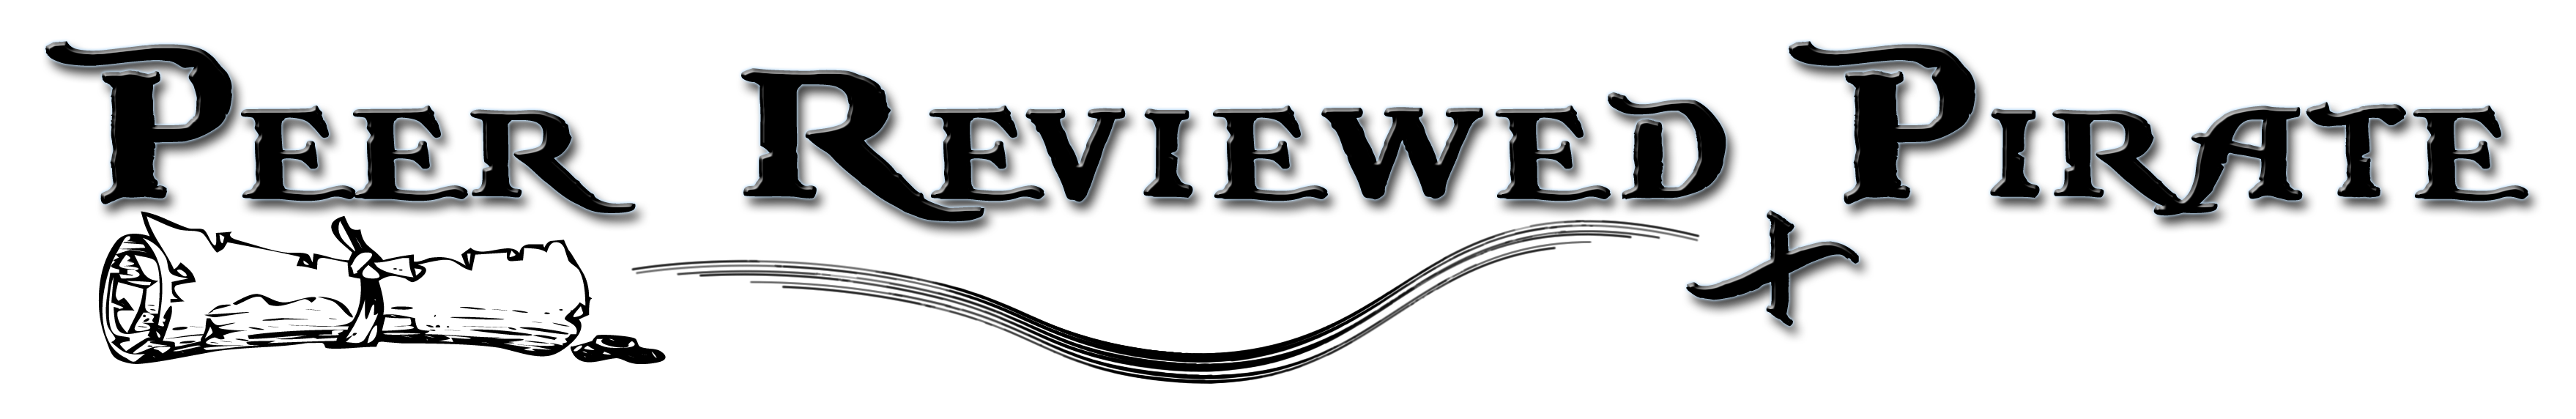
\includegraphics[width=\linewidth]{../images/banner/PRP-banner.png}
	%\HorRule\vspace{10pt} % Horizontal rule before the title
	\fontsize{32}{36}\usefont{OT1}{phv}{b}{n}\selectfont % Helvetica
	\color{DarkBlue} % Text colour for the title and author(s)
}


\posttitle{\par\vskip 3pt} % Whitespace under the title

\preauthor{} % Anything that will appear before \author is printed

\usepackage{multicol, etoolbox}
\setcounter{tocdepth}{3} %set depth of printed table of contets.
\makeatletter
\patchcmd{\l@section}
{\hfil}
{\leaders\hbox{\normalfont$\m@th\mkern \@dotsep mu\hbox{.}\mkern \@dotsep     mu$}\hfill}
{}{}

\renewcommand\tableofcontents{%
	\begin{multicols}{2}
		\@starttoc{toc}%
	\end{multicols}%
}
\makeatother %print dots in sections in toc.

\postauthor{ % Anything that will appear after \author is printed
	\vspace{3pt} % Space before the rule
	\begin{center}
		\fontsize{16}{18}\usefont{OT1}{phv}{b}{n}\selectfont % Helvetica
		\color{DarkBlue} % Text colour for the title and author(s)
		https://PeerReviewedPirate.github.io/ \\
		Issue \Version - \DateToUse
	\end{center}
	\vspace{3pt} % Space before the rule
	\par\HorRule % Horizontal rule after the title
	\vspace{5pt} % Space after the title section
	\vspace{5pt} % Space after the title section
	\begin{minipage}{\linewidth}
		\renewcommand\contentsname{} % the empty name for toc
		\begingroup
		\let\clearpage\relax
		\vspace{0.5cm}
		\small\tableofcontents
		\thispagestyle{fancy}
		\endgroup
	\end{minipage}
}

%----------------------------------------------------------------------------------------
%	ABSTRACT
%----------------------------------------------------------------------------------------

\usepackage{lettrine} % Package to accentuate the first letter of the text (lettrine)
\usepackage{fix-cm}	% Fixes the height of the lettrine

\newcommand{\initial}[1]{ % Defines the command and style for the lettrine
	\lettrine[lines=2,findent=4pt,nindent=0pt]{% Lettrine takes up 3 lines, the text to the right of it is indented 4pt and further indenting of lines 2+ is stopped
		\color{DarkBlue}% Lettrine colour
		{#1}% The letter
	}{}%
}

\usepackage{xstring} % Required for string manipulation
	
\usepackage{stfloats} % Allows the H option in figures.

\newcommand{\abstract}[1]{
	\begin{figure*}[t]
		\centering
		\begin{minipage}{0.9\textwidth}
			\HorRule\color{black}\vspace{-6pt}
			\StrLeft{#1}{1}[\firstletter] % Capture the first letter of the abstract for the lettrine
			\initial{\firstletter}\textbf{\StrGobbleLeft{#1}{1}} % Print the abstract with the first letter as a lettrine and the rest in bold
			\HorRule
		\end{minipage}
	\end{figure*}
}

%----------------------------------------------------------------------------------------
%	Section Titles
%----------------------------------------------------------------------------------------

\setcounter{secnumdepth}{0}

\usepackage{titlesec}
\titleformat{\section}
{\normalfont\Large\bfseries}{\thesection}{1em}{}[{\titlerule[0.8pt]}]

%----------------------------------------------------------------------------------------
%	BIBLIOGRAPHY
%----------------------------------------------------------------------------------------

\usepackage[backend=bibtex,style=authoryear,natbib=true]{biblatex} % Use the bibtex backend with the authoryear citation style (which resembles APA)

\addbibresource{../resources/references.bib} % The filename of the bibliography

\usepackage[autostyle=true]{csquotes} % Required to generate language-dependent quotes in the bibliography

%----------------------------------------------------------------------------------------
%   FANCY BOXES
%----------------------------------------------------------------------------------------

\usepackage{tikz}
\usetikzlibrary{shapes,snakes}
\usepackage{amsmath, amssymb}
\usepackage{polynom}

\usepackage{wrapfig}

\usepackage{lipsum}

% Define box and box title style
\tikzstyle{mybox} = [draw=blue, fill=cyan!20, very thick, rectangle, rounded corners, inner sep=15pt]
\tikzstyle{fancytitle} =[fill=LightBlue, text=black, draw=blue, very thick]

\newcommand{\bluebox}[3]{
	\begin{wrapfigure}[#3]{r}[\dimexpr\columnwidth+\columnsep\relax]{11.5cm}
		\resizebox{12cm}{\height}{
			\begin{tikzpicture}
				\node [mybox] (box){%
					\begin{minipage}{0.70\textwidth}
						#2
					\end{minipage}
				};
				\node[fancytitle, right=10pt] at (box.north west) {\hspace{2pt}#1\hspace{2pt}};
				%\node[fancytitle, rounded corners] at (box.east) {$\clubsuit$};
			\end{tikzpicture}%
		}
	\end{wrapfigure}
}

\usepackage[framemethod=TikZ]{mdframed}
	
\newenvironment{fancybox}[2][]{%
	\ifstrempty{#1}%
	{\mdfsetup{%
			frametitle={%
				\tikz[baseline=(current bounding box.east),outer sep=0pt]
				\node[anchor=east,rectangle,fill=LightBlue]
				{\strut};}}
	}%
	{\mdfsetup{%
			frametitle={%
				\tikz[baseline=(current bounding box.east),outer sep=1pt]
				\node[draw=blue,anchor=east,rectangle,fill=LightBlue,rounded corners]
				{\hspace{3pt}#1\hspace{3pt}};}}%
	}%
	\mdfsetup{innertopmargin=5pt,linecolor=DarkBlue,%
		linewidth=1pt,topline=true,,%
		frametitleaboveskip=\dimexpr-\ht\strutbox\relax
	}
	\begin{mdframed}[backgroundcolor=cyan!20]\relax%
		\label{#2}}{\vspace{4pt}\end{mdframed}}
	
% for adjustwidth environment
\usepackage[strict]{changepage}

% for formal definitions
\usepackage{framed}

% environment derived from framed.sty: see leftbar environment definition
\definecolor{formalshade}{rgb}{0.95,0.95,1}

%\newenvironment{formal}{%
%	\def\FrameCommand{%
%		\hspace{1pt}%
%		{\color{DarkBlue}\vrule width 2pt}%
%		{\color{cyan!20}\vrule width 4pt}%
%		\colorbox{cyan!20}%
%	}%
%	\MakeFramed{\advance\hsize-\width\FrameRestore}%
%	\noindent\hspace{-4.55pt}% disable indenting first paragraph
%	\begin{adjustwidth}{}{7pt}%
%		\vspace{2pt}\vspace{2pt}%
%	}
%	{%
%		\vspace{2pt}\end{adjustwidth}\endMakeFramed%
%}

\interfootnotelinepenalty=10000 % Keeps footnotes on one page

\newenvironment{formal}{%
	\def\FrameCommand{%
	{}%
	{}%
}%
\MakeFramed{\begin{mdframed}[backgroundcolor=cyan!20, bottomline=false, topline=false, rightline=false, linewidth=2pt, linecolor=DarkBlue]\relax\advance\hsize-\width\FrameRestore}%
\noindent\hspace{-4.55pt}% disable indenting first paragraph
\begin{adjustwidth}{}{7pt}%
}
{%
	\end{adjustwidth}\vspace{2pt}\end{mdframed}\endMakeFramed%
}

\usepackage{tikz,lipsum,lmodern}
\usepackage[most]{tcolorbox}

\newcommand{\imagebox}[2]{
	\begin{tcolorbox}[enhanced,frame style image=../images/blue-abstract.jpg, 
		opacityback=0.75,opacitybacktitle=0.25,
		colback=blue!5!white,colframe=blue!75!black,title=#1]
		#2
	\end{tcolorbox}
}


\newcommand\blankfootnote[1]{%
	\let\thefootnote\relax\footnotetext{#1}%
	\let\thefootnote\svthefootnote%
}



\AtBeginBibliography{\small} % Makes the references smaller. % Specifies the document structure and loads requires packages

%----------------------------------------------------------------------------------------
%	ARTICLE INFORMATION
%----------------------------------------------------------------------------------------

% The article title
\title{\begin{center}Pirates, Conspiracies, And The Tragedy Of COVID-19\end{center}} 

\author{
	\begin{center}
		\authorstyle{Author(s): Antonius Torode\textsuperscript{1,2,3,4,5}}\\ % Authors
		\vspace{0.5cm} % Space before institutions
		\textsuperscript{1}\institution{Engineering Scientist Associate, University of Texas: Austin}\\
		\textsuperscript{2}\institution{Degree in Biblical Studies, Ambassador Bible College}\\ 
		\textsuperscript{3}\institution{Bachelors of Physics, Michigan State University}\\ 
		\textsuperscript{4}\institution{Bachelors of Mathematics, Michigan State University}\\ 
		\textsuperscript{5}\institution{https://torodean.github.io}\\ 
	\end{center}
}

\date{} % Add a date here if you would like one to appear underneath the title block, use \today for the current date, leave empty for no date

%----------------------------------------------------------------------------------------

\begin{document}

\maketitle % Print the title

%Copywrite page
\onecolumn
	%% copyrightpage
	\begingroup
	\footnotesize
	\parindent 0pt
	\parskip \baselineskip
	\textcopyright{} 2022 Antonius Torode \\
	All rights reserved.
	
	The articles of this work may be distributed freely. 
	
	
	\textbf{About this document:} The Peer Reviewed pirate is a publication containing various information. Each article will be published to the main website when completed. On occasion, small typos, grammar, or spelling errors will be caught that were not be found in the initial editing stages. If this occurs, they will be corrected and a new version will be uploaded with the fixes. The date of the document will not change from it's original. It is also possible that larger errors may be found. One of the main purposes of this document is to apply the scientific approach and dissemination of information. For this reason, other additions may be added as feedback from readers is received. \textcolor{Red}{If this is the case, these additions will be added in red lettering and a small note will be added to the title page stating that there was an update with a date attached.} This is done for potential referencing situations. The format of this document is defined below. This copywrite/about page is subject to potentially change in later versions.
	
\vspace{0.5cm}
	
\begin{framed}[.5\textwidth]
	\begin{minipage}{\linewidth}
		\section*{Article Title}
		Each issue contains multiple articles. Each article is it's own thought and may or may not be related to the other articles.
		
		\hspace{1em}\subsection*{Section}
		
		An article may have multiple sections. Each section should be related to the overall article focus but may provide a logical separation between the various elements of the article.
		
		\hspace{1em}\subsubsection*{Sub-section}
		
		Sub-sections are simple dividers that may be used within the various sections. This is to simply provide the reader with shorter parts to read or stopping points throughout. Each article will be concluded with the symbol below.
		
		\sectionEnd
		
		\section*{References}
		The references are provided at the end of each volume for all of the articles it contains. They are in alphabetical order.
	\end{minipage}
\end{framed}


	\vspace{1cm}
		
	The original maintainer of this work is: Antonius Torode. \\		
	The current maintainer of this work is: Antonius Torode. \\
	Chief Editor: Antonius Torode\\		 		
	Published by Antonius Torode. 
	
	\textbf{Hosted at}: https://PeerReviewedPirate.github.io/
	
	
	\vfill
	
	\textbf{Citation:} \\
	\hspace*{2em} Torode, A.\\
	\hspace*{2em} <Article Title>. \\
	\hspace*{2em} Peer Reviewed Pirate. \\
	\hspace*{2em} \DateToUse. \\
	\hspace*{2em} Volume. \Version. \\
	\hspace*{2em} https://PeerReviewedPirate.github.io/
	
	\endgroup
	\clearpage
\twocolumn


%----------------------------------------------------------------------------------------
%	ABSTRACT
%----------------------------------------------------------------------------------------

\abstract{Being the first of many volumes in the Peer Reviewed Pirate series, this issue will serve to outline introductory details and introduce the reader to the various elements that will be included. It begins with a short introductory section about this publication followed by some useful tools when looking for, examining, and expressing information with a brief introduction to conspiracy theories. Following this, a summary of various COVID-19 research I have collected since the start of the current pandemic with some unique connections that I have not seen elsewhere.}

%----------------------------------------------------------------------------------------
%	ARTICLE CONTENTS
%----------------------------------------------------------------------------------------

\section{About The Peer Reviewed Pirate}

The Peer Reviewed Pirate is a monthly publication akin to an academic journal. The main difference being that it is self published and primarily contains writings of a single author similar to a blog. Like most of my other projects, the primary reason for creating this is to improve upon my own skills and knowledge. This will serve as a place where I can combine thoughts and information in a coherent manner and share those with others. The contents will vary drastically but pertain primarily to current day events and other things that the author(s) have been researching and thinking about. The goal, as it pertains to sharing information, is to do such in an efficient and effective way. The topics covered in this publication include but are not limited to the following.

\subsubsection*{Historically significant accounts}
It is important to understand history in order not to repeat the mistakes it demonstrates. Through studying the past, we can learn valuable techniques for approaching the future. We can understand what things could occur to us and gain the knowledge from previous generations.

\subsubsection*{Useful information}
Often times it is very easy to learn of just generally useful things. Without sharing these tidbits of knowledge, how will it be preserved? It is important that if we understand something and there are others willing and wanting to learn it, we help share the knowledge. By sharing information, there becomes a larger number of minds that can all think about it from various perspectives, potentially giving us advancements and furthering the onset of new ideas.

\subsubsection*{Important life lessons}
Through our own personal experiences, each and every one of us learns valuable lessons. It is important to share these with others to limit repeated mistakes and share wisdom that we each learn.

\subsubsection*{Mathematics}
This has always been a passion of mine. I believe mathematics is an important tool that can be used to better understand the world around us. It contains concepts that can be applied to improve our daily lives and can lead us to astonishing results about our surroundings. One of my past co-workers from my college days once jokingly said ``everyone should be required to get a master's in mathematics''. Although most would greatly disagree, the underlying reasoning for this is very valid. Along with learning mathematics, one has to learn logic, reasoning and problem solving. These are skills that would benefit anyone and are lacking in many.

\subsubsection*{Technological advancements}
The world around us is exponentially increasing when it comes to technological advancements. In just the span of a generation, one can lose sight on all the new advancements and not be able to maintain their ability to learn about new technologies effectively. This is often seen with the current older generations. It is important to understand new discoveries, advancements, and the potential impacts they can have on the world and our culture around us.

\subsubsection*{Thought provoking concepts}
These are simply ideas that are meant to illicit the reader to think about things in new and unique perspectives. I find that with all the technological distractions we have today, there is a lot less time thinking and understanding everything we hear. I once had a friend who wanted to listen to a podcast I listened to at 1.5x speed. Although this is probably simple to do for some, I would argue that those aren't podcasts worth listening to. It is often that I find myself expanding and coming up with new ideas by simply contemplating and questioning what was heard. This requires thinking and analysis and is not something that is easier to do when speeding through information. Like the ol' adage states, it is quality, not quantity. 

\subsubsection*{Biblical history and concepts}
As someone who has spent a large portion of their life dedicated to studying the historical context and wisdom contained within the Bible, I feel it is important to share that knowledge. Although many would disagree and think it has no relevance, I find that it perfectly complements the knowledge of our age and provides wisdom that holds firm with current and new `discoveries'. Whatever your religious beliefs, it is important to gain an understanding from all perspectives. To dismiss something because of its origin simply shows a lack of openness and an unwillingness to learn new perspectives.


\subsubsection*{Nutrition and Cooking}
As humans, health and nutrition are important to both physical and mental capabilities. Much of the information on health and nutrition is based on biases of corporations who only benefit from it. Other information is clearly understood and yet so many have an opposite understanding. This is a topic that should be understood and continually studied by all in order to maintain a healthy life. As for cooking, it is a lot easier to maintain a nutritious diet if you enjoy what is eaten. An essential skill that is not taught in traditional schools is that of cooking. Over the years, I have found some techniques and recipes that think should be shared and could be beneficial to all.


\subsubsection*{Much more}

I plan to cover the written topics in a manner that is from a logical and scientific perspective but also try to look at things from new points of view. For the reader, I hope to give the sense of information from the perspective of a physicist. In today's world, which some would say is chaos and mayhem, it can be vastly beneficial to take a step back and view things from a logical perspective. With most topics, you can find arguments for and against them. With most political subjects, you can find extremes in either direction. What's often missing is a balanced perspective that tries to identify the truths of multiple perspectives and objectify reality. 

In today's society, podcasts are becoming increasingly the go to information sources for the younger generations. Those who work towards a scientific understanding don't stop at just listening, but then further research and confirm things they hear from these audio sources. This is the aspect of research that relies on reading and finding reputable sources. It is my hope that this publication becomes a reliable source that can be used for reference and citation in other pieces. I hope to provide coherent written explanations for those looking to further their understanding and potentially write something similar themselves.

\subsubsection{Why Pirates?}

A pirate typically has a negative connotation associated with it. This is not what I am going for. In today's society, it seems that there is an increasing pattern of information silencing and suppression that opposes various political agendas. The desired idea of a ``pirate'' here is one of opposing that authority and providing information in which suppression could potentially be desired. In a system where ideas which challenge the status quo often vanish or never make it to the public eye, I believe it is beneficial to bring them into the light. There is also a large emergence of relying on exclusively peer-reviewed information by some groups. Although this is not wise to be exclusive about this, peer-reviewed sources are designed such that they can provide a more trustworthy data source (not saying this is always the case). Thus, the desired goal of the ``peer reviewed pirate'' is to be a name of opposition the political agendas that can be trusted.



\subsection{How To Contribute}

It takes a lot of time to compile, analyze, and write about any research topic. It takes even more time to write about topics that are non-trivial or have many aspects to them. Unfortunately, it is not easy to balance everyday life and the time required to do this in a thorough way. For this reason any financial contributions would not be rejected as they would help free up time. Alongside this, any articles that anyone would wish to be submitted for review and possible addition to the Peer Reviewed Pirate should be sent to the author\footnote{Contact information can be found in the website listed in the author's section.} and they will be considered for addition.














\sectionEnd

\section{Clear Explanation Through Precision of Speech}

\begin{quotation}
	``If you don't tidy your room, then you won't get any ice cream." \citep{HowToThinkLikeAMathematician}
\end{quotation}

This is a quote from one of my undergraduate mathematical textbooks. Not only that, but to me it is one of the most important quotes in the entire book. Not because of what it says, but rather what it represents. On the surface, many people will interpret this as getting ice cream if you tidy your room. However, this statement does not say anything about what will happen if you actually tidy your room. On the contrary, it only explains what will happen if you \textit{do not} tidy your room. Apples and oranges right? Well, apples and oranges are very different fruits, as is this statement from one stating what would happen if you did tidy your room.

The distinction here is subtle, though pointing it out is necessary. It is commonplace for people to be misunderstood in day to day language. Whether this is from their own imprecision of speech, from a wrong interpretation, or perhaps a combination of both, misunderstandings can cause great turmoil - causing frustration, pain, or even detrimental mistakes. For this reason, it is best to adapt behaviors that support being both precise in speech and trying to precisely understand others. 

\begin{formal}
	 ``Even things without life, whether flute or harp, when they make a sound, unless they make a distinction in the sounds, how will it be known what is piped or played? For if the trumpet makes an uncertain sound, who will prepare for battle? So likewise you, unless you utter by the tongue words easy to understand, how will it be known what is spoken? For you will be speaking into the air." - 1 Corinthians 14:7-9 (NKJV)
\end{formal}

Mathematics and Engineering, by design, are languages in which precision is built in and things are defined in such a way that they cannot be misunderstood (to the extent that they are interpreted correctly). Imagine a blueprint design of a bridge. It should be the case that no matter who looks at the blueprint to build the bridge, the end result of construction should always be the same (given the same material availability and no human mistakes are made). If it were not the case and the blueprints could be interpreted in different ways, then there would be no telling how said bridge would turn out. If an engineer specifies a bridge support beam should be 10 meters long (given standard room temperature and pressure) but someone uses one at 12 meters long instead, there would be issues with how all the other pieces fit together. 

English (and similarly, other languages), within the context of its cultural influence, is not designed in the same way. However, it has the capability to be utilized in such a way. In the context of mathematics, it is often expressed with a language representation. There are predefined set rules to use when expressing mathematical expressions in a written language that are defined such that it cannot be misinterpreted. With our example above about not getting ice cream, there is no room for misinterpretation given you read and interpret the statement as it is written.

\subsection{The Mis-calibration Of The Hubble Telescope Lens}

When the Hubble Telescope was launched, the first images NASA began receiving from it were blurry. The quality was much lower than what was expected. Upon a thorough investigation, they determined that the issue was caused by an error in the primary mirror of the telescope. This error was on the order of 1 micron in size (about one 50$^{\text{th}}$ the width of a human hair). In 1993, astronauts had to travel into space and correct the issue by installing The Corrective Optics Space Telescope Axial Replacement (COSTAR) instrument - which corrected the issue in a way analogous to how a pair of eye glasses work \citep{HubbleMirrorFlaw}. This error was incredibly small, though the lack of precision in the machining of this telescope lens led to very poor results for its performance. It is not always immediately obvious how a small error could affect the outcome of something. For this reason, maintaining precision is greatly desired. This applies as much to speech as it does for simple engineering.

\subsection{Think Rationally With Proofs}

In mathematics, we can determine absolute truths using what is referred to as proofs. Through a set of logical methods, approaches, and applying definitions, various statements can be proven true. If something is proven true, it will always be true. Therefore, if something can be shown to not hold true, it has not been proven. There is a very distinguishable difference between evidence that supports and idea or statement and a proof. The former is simply showing that it may be true, or hold in some situations. When using modern day language, people often look for proofs with respect to counter arguments, `facts' and information they hear. In many cases, statements that support an argument are mistaken for proofs and thus arguments are thrown out or misunderstood. This is very commonly seen with communication found on the internet.

One tool often used by mathematicians is the proof by contradiction. This is likely one of the easiest ways to prove something is true or false. The premise of a proof by contradiction is that if a statement leads to a contradiction by applying sound logic, it cannot be true. For example, let's say $x$ is a positive integer - meaning $1,2,3,etc...$ (represented as $x \in \mathbb{N}$) if I were to say $x=5$ and $x=6$, this is a contradictory statement, for $x$ cannot be both 5 and 6, because 5 does not equal 6. Written as a mathematical contradiction proof, this would be as follows.

\begin{fancybox}[Example of Proof By Contradiction]{}
	\textit{\textbf{proof.}} Assume for $x \in \mathbb{N}$ that ``$x=5$ and $x=6$''. If $x=5$ and $x=6$, then $5=6$. This is a contradiction, as 5 does not equal 6. Thus, we can conclude that ``$x=5$ and $x=6$'' is false\footnote{This further implies that either $x\neq5$ and/or $x\neq6$.}. $\square$
\end{fancybox}

The concept of a proof by contradiction can easily be applied to speech, though often more subtle than the mathematical examples. When making an argument or statement, it is important to avoid contradictory statements. This is easier to do if what you are saying is true and accurate. Similarly, when listening or reading, it is important to watch for and identify contradictory statements. This is a simple way to determine if what you are reading is both accurate and reliable. When you stumble across contradictory information, you may need to re-evaluate whether you are getting your information from a reliable source. When you are in a conversation, it may be necessary to ask clarifying questions as it is often the case that contradictions arise unintentionally due to simple misspeaking or using the wrong words. 

I have had this happen on many occasions with my own speaking, where I will use the completely wrong word for something when another word was meant - just part of being human. An alternate distinction can come when people change their mind. When it comes to human interactions, you can typically distinguish between various cases such as this, though it is important to note that not all contradictory statements are actual contradictions in this context. When someone changes their mind, the new statements supersede the former. Contradictions arise when multiple things (statements, phrases, actions) are believed to hold true, but they contradict. The way in which these can be subtle varies by situation. It may be the case that someone says two things that seem contradictory, but in two different contexts - which would not be contradictory. It may also be the case in which someone says something and then does the opposite. Hypocrisy is a type of contradiction to the self.

\subsection{The Subtle Distinctions In Speech}

\begin{quotation}
	``If you tidy your room, then you may or may not get ice cream."
\end{quotation}

The above statement is only slightly different from our original, though the meaning is very contrasting. Where the original statement only explained what would happen if you did not tidy your room, this one explains what would happen if you do. The way it is written, it could seem as though it has the same meaning as the original. Since the original did not say what would happen if you tidied your room, the opposition would be that anything could happen in that situation. The subtle distinction here is that the way this statement is written, it says nothing about what would happen if you do not tidy your room. Therefore, it could very well go along with the statement ``if you don't tidy your room, you will get ice cream" (although in context it doesn't make much sense, it is still logically consistent). 

In general, you don't have to think hard about the subtle distinctions like this example. There is usually an element of context which can bring light to the meaning of a phrase. For example, if you were to state ``If you tidy your room, then you will get ice cream," then there is a clear reward for a task given. For a native English speaker, there is not much room for misinterpretation here. On the contrast, if you use our original statement, ``If you don't tidy your room, then you won't get any ice cream," it could be taken more as a threat. As we've already stated, and is commonly done, this could be taken as getting ice cream for tidying your room. However, without lying, this is a subtle way to convince someone to tidy their room, with a potential promise of ice cream. I am repeating this concept because it is a tactic of a commonly used tool - deception. 

Rather than a silly example about cleaning rooms, this principle should and can be applied to information all over. In particular, scientific writings and legal documents are typically designed in such a way that they are precise. I will demonstrate applying what is discussed here with one random example found while flipping through my notes. On August 23, 2021, the FDA approved the Pfizer-BioNTech COVID-19 vaccine to be marketed as Comirnaty. In an FDA news release, they outline some minor details of their trial that was used to make this determination. Within the news release, they state

\begin{quotation}
	``the agency analyzed effectiveness data from approximately 20,000 vaccine and 20,000 placebo recipients ages 16 and older who did not have evidence of the COVID-19 virus infection within a week of receiving the second dose." \citep{FDAApprovesVaccine}
\end{quotation}

The important part of this is when it states ``who did not have evidence of the COVID-19 virus infection within a week of receiving the second dose." As of August 23, there are presumably very accurate ways to determine whether someone has SARS-CoV-2. Therefore, why would ``evidence'' be used rather than just ruling out those who had COVID-19. This, like any other scientific piece of writing is likely deliberate. Evidence can simply mean ``an indication or sign" \citep{dicionary}. At first read, this seems as though they threw out all the people who got COVID-19 within a week of receiving their second dose, however evidence of changes this to be anyone who showed any sign of having COVID-19 after their second shot. The most important part of this distinction comes from the context of this situation. The majority of side effects that have been reported for the vaccine are similar to the symptoms or side effects of COVID-19 itself \citep{ComirnatyFactSheet}. Furthermore, these symptoms tend to occur most often within a week after the second dose. This demonstrates that the way this is stated, it could potentially be used to rule out adverse events from the vaccine itself and thus drastically skew these trial results! If this was the case, it would be a prime example of deception through precise speech (or imprecise in that matter). Of course this is not saying that's the case, though it certainly suggests it could be. Without further information, there is no way to conclude the full meaning of the quotation. If you aren't precise, you may not be understood. 

Through these examples, I've demonstrated that precision of speech can make a vast difference in meanings and understanding. It is therefore important to maintain precision in speech and be sure to stay consistent throughout words, actions, context, and anything else that can lead towards an interpretation. It is also important to understand that we are all human and incapable of perfection. Therefore, take into account the imprecision of others and use clarifying questions when needed. Just as a computer chip must be made precisely, so too should we try to be understood. Precision is not just a tool for the mathematician.














\sectionEnd

\section{To Identify Robust Sources}

A large part of researching any topic is determining what sources are trustworthy and which are not. It is a common retort that a source is just simply untrustworthy and therefore the person using it to support their statements is simply wrong. I once had someone tell me that they can only trust peer-reviewed articles published on ncbi.nlm.nih.gov and when I sent them an article from that supporting my statements, they replied with a TikTok\footnote{...}.

The process of peer-reviewing is designed to assess the quality of articles that make it to publication. When an article is submitted to a journal, the editors will forward the article to other qualified individuals in the field. The article will undergo evaluation with certain standards defined by the journal editors. The peer-reviewers are typically to check the methodology that the article uses as well as validity of the research. Revisions may be suggested to the original author, and when the review process is completed, the paper will either be published to the journal or rejected. 

The peer-review process is not perfect and thus there is a possibility that a peer-reviewed paper can be retracted after publication. This happens when other experts in the field find errors in the paper or various other reasons. In theory, the peer-review process would be enough to consider the article as robust and trustworthy. In practice, this is not the case, which is why articles often get retracted. Despite this, peer-reviewed articles are a great place to look for information compared to many others. There are a few things that should be considered when finding resources that can help improve the accuracy of the information you find.

\begin{itemize}
	\item Find multiple sources that say or support the same thing.
	\item Find journals that have high standards for quality and reviewing processes.
	\item Be wary of the author affiliations. Often times a study can be performed in such a way that will bias the results towards a desired outcome.
	\item Don't confuse red flags with explainable issues\footnote{I once had someone reject a paper I sent them because there was a typo. They did not realize that the author was Japanese and English was not their primary language - which likely meant the reviewers weren't either.}. 
\end{itemize}

A common phrase uttered is that you can find information supporting anything on the internet. Unfortunately, this is generally true. Anyone can create a free website and post whatever they want on it. Even if information on something didn't exist, it would only take a mere matter of seconds to create a web page that has it. The media definitely doesn't help when you have information covered in such a way only to support specific narratives. The remedy to this is simple. Avoiding opinion pieces and going straight to the source is generally the easiest way to get the most accurate information. Similar to the game of telephone, each time something is portrayed, it can have information removed or added to it. When dealing with sources that aren't peer-reviewed, you can still find valid and useful information, but you have to be much more careful. A few things you can consider when looking for information follows.

\begin{itemize}
	\item Look at the source of the information. When finding a piece of information, look for the sources they use. A trustworthy source should have more merit than an untrustworthy one. 
	\item Look for any biases. Even the most trustworthy source could hold an inherent bias.
	\item Maintain consistency and avoid contradictions. True information should hold consistent and not contradict itself.
	\item Question everything you see. Even if you immediately believe a piece of information, you should consider flaws and possible questions to ask about it.
\end{itemize}

When looking at resources, you should also consider the contents and layout of the information itself. If a piece of information is not well written, it is possible that it was meant to be written that way. If a piece contains logical inconsistencies, it may not be the best source to be using. If a piece contradicts itself, it may be simply spouting nonsense. On the other hand, it may be that there is a simple misunderstanding from the reader. 

Over the course of the past year, the paradigm of spreading, posting, and sharing information has drastically changed. There has been a large prevalence of misinformation as well as information being censored and removed. Censoring information is never a good idea because it is often found that it had merit after the fact and the act of censoring has given that piece a bad reputation (often also the purpose). `Fact-checkers' have become widely thought to do just what their name suggests - fact check. Unfortunately many of those who actually read the fact check articles as well as the original sources that they `check' realized that they are not very good at this and seem to be only `checking' in the sense of debating things to fit a specific narrative (this is not my opinion, but rather an observation by many). In recent news releases it was shown that Facebook admitted that fact-checkers used by the site are merely opinions\footnote{``they constitute protected opinion." - U.S. District Court, Case 5:21-cv-07385-VKD, Document 27, Filed 11/29/21, Page 10 of 32}.

The last thing I'd like to address is context. Quotes can be a great place to find information. Quotes are easy to take out of context, however. When finding sources with quotations, be sure that they are not taken out of context. Look into the sources and determine the context yourself. This is most often done with biblical scriptures. Often times without knowing, it is incredibly easy to take Bible scriptures out of context. One reason is because the English translation of a verse or cultural setting it was written in have an entirely different meaning than the original. One simplistic example is found in Philippians 3 verse two. It starts out by ``beware of dogs", though has nothing to do with actual dogs. 

These ideas and concerns with sources are just the tip of the iceberg. With all research, consider these steps in finding robust and trustworthy sources. Look for direct sources, make your own opinions, and keep an open mind as to information that is presented as well as questioning it thoroughly.











\sectionEnd


\section{The Surface Level Depth Of Conspiracy Theories}

Conspiracies are a hot topic of discussion among many groups. Just the other day, this topic came up in a conversation among church brethren. A familiar phrase was uttered, which I have previously heard from many different people in regard to the subject matter. That phrase was effectively ``conspiracies don't actually exist, because people are not capable of organizing them.'' One thought behind this is that human beings are not intelligent or organized enough to plan and carry out conspiracies. Before continuing, it is important to define a conspiracy. 

\begin{fancybox}[Definition(s): Conspiracy]{}
	\begin{enumerate}
		\item The act of conspiring.\blankfootnote{Definitions from \cite{dicionary}}
		\item An evil, unlawful, treacherous, or surreptitious plan formulated in secret by two or more persons; plot.
		\item Any concurrence in action; combination in bringing about a given result.
	\end{enumerate}
\end{fancybox}

Another simple example some use to support the claim that conspiracy theories don't exist is that if they were to exist, there would often be too many people who would have to keep the secrets in order for it to not go public. This is then seen as unfeasible. As someone who has had to sign countless nondisclosure agreements within my employment career, along with having an active secret security clearance, I would argue against this. In many cases, the ramifications of breaking a contracted nondisclosure agreement would be detrimental to the livelihood of an individual. When dealing with classified information, there is always a 'need to know' mentality. Unless information is needed for the task at hand, you are not privy to it. Furthermore, it is often not a piece of information that is classified by itself, but rather the connection of multiple sources combined that is classified. In other words, you can have many un-classified pieces of information, but a certain connection that relates them could be what is classified. Together, these make the opportunity for a conspiracy theory very feasible.

Conspiracies are often thought of in a negative connotation. For this reason, the second definition seems fitting. To think that conspiracies are non-existent is a simple matter of ignorance. Throughout history, there have been a large number of conspiracies that have been uncovered. The easiest way to prove that conspiracies do exist is to thus simply demonstrate that one has before existed. 

\subsection{The Phoebus Cartel}

A well-known conspiracy by many can be referred to as \textit{The great light bulb conspiracy} \citep{IEEELightbulbConspiracy}. In December of 1924, a group of international businessmen (in this case, leading representatives from all of the major light bulb manufacturers) gathered in Geneva for a meeting where they founded the Phoebus cartel. Their vision was to artificially engineer the need for a greater light bulb market through controlling production quotas, suppressing technological advancement, and even reducing the lifespan of the available incandescent light bulbs.

The Phoebus cartel had successfully reduced the average age of the light bulb to roughly 1,000 hours for the household bulb. This was reduced from the 1,500 to 2,000 hours that was previously common at this time. The cartel was motivated by profits and increased sales which began the well known production strategy of \textit{planned obsolescence}. Although this tactic is of potential interest to isolated parties in order to facilitate collusion and potentially higher profits, the monopoly or explicit collusion method is far superior \citep{Strausz2008Collusion}. The only difference being that the latter is two or more parties working towards a common goal, such as the Phoebus cartel, and hence fitting perfectly with definition 2 of a conspiracy.

\begin{formal}
	Fun fact: The worlds oldest burning light bulb has been illuminated for over 120 years \citep{LightingTechnology,centennialLight}!
\end{formal}

\subsection{Planned Obsolescence}

Although it would be wonderful and seem reasonable to have products created to last, it is not `economically' feasible (what?). By definition, economically should mean ``in an economical manner; not wastefully; not extravagantly; prudently.'' However, in a world driven by the exchange of money through goods and services, this is not necessarily the case for a good business model and thus the desired `economics'. This is easily demonstrated - for if people do not buy many products, there will be little need for workers to produce those products, and thus there will be a lack of wage earnings due to limited workers. This outcome would not be good if you are trying to make profits through selling goods. This was even seen to be a large factor in the great depression, which some suggested to resolve through the direct use of planned obsolescence \citep{london1932}. 

It is commonly referred to by economists or businessmen as progress when sales increase and higher profit margins are attained by an entity, though the contrary would be argued from the stance of sustainability and durability. Given a set of goods, the most sustainable and efficient approach would be to create them such that they would not need to be replaced and last indefinitely - whether through replaceable upgrades or just intrinsic durability and function. This would ensure that there is no need for increasing sales over time, as there would potentially eventually be a number of goods reached to suffice the need of everyone alive, and only to increase when the population does accordingly. This of course could also conflict with technological advancement, which is where upgrade-able and adaptable products could play a role. This is the contrary view of planned obsolescence, as a decrease in demand would result in a corresponding decrease in sales and thus revenue for the entity of production.

Imagine for a moment, that every consumer purchased the new apple iPhone when it was released. The corporation of Apple would be very pleased, as sales would skyrocket. Therefore, living in a world as we do that is driven by goods and services, planned obsolescence is a benefit for corporations and other entities. It is commonly utilized among people still to this day. For many, this is the underpinning of conspiracy theories by corporations all around. Although good for businesses and profit, what are the ramifications of such a system? Is planned obsolescence a good thing and thus not capable of falling within the conspiracy theory title? Some sources would certainly suggest that this is a good thing and a necessary condition for technological progress \citep{PlannedObsolescenceasanEngineTechnologicalProgress}. However, what would happen to all those replaced iPhones? Other sources point out the negative consumer effects, accelerating destruction and higher levels of ecological spoilage introduced by the process \citep{ConsumptionPlannedObsolescenceAndWaste}.

Over time, industrial practices have improved both efficiency and the environmental impact of production. In many cases this was forced due to production causing drastic ecological damage and government or community intervention. In other cases. these naturally came about as technological advancements were made. Despite this, it has become increasingly clear that sustainable development which remains within the ecological limits cannot be reached by such interventions \citep{LiveBetterbyConsumingLess}. Both these negative impacts that planned obsolescence can cause, and the secrecy or privacy of groups that design the systems in this way make this a perfect example of not only one conspiracy theory, but many - with respect to each different group that follows such a process.

\subsection{Zugzwang: The Death Of A Conspiracy}

A conspiracy theory can be made analogous to a game of chess. The end goal is to checkmate the opponent's king. However, the path in which this is done varies depending on the opponent's moves. If you are playing with someone of similar level, you would not have the entire game planned out. But rather, you would think a few moves ahead and try to understand what your opponent is thinking as well. Some players who have studied chess will have a better idea of what will work and how to setup a preferred end game. The same is true for the world around us. It is not hard to conceive that a group who studies history and has the resources to work towards a goal, that they could not design and implement a plan towards their checkmate. As scenarios change, the plans are modified accordingly, with that end goal still in mind. 

When one player is up to make their move, but they have no good moves (every move would worsen the position), this is referred to as zugzwang. When a lot of things happen that go against a conspiracy theory, it will become more difficult to adapt and adjust to the changes. Eventually, there will be no beneficial moves left and the conspiracy will crumble. With the Phoebus cartel, details of the conspiracy were very slow to emerge and some even became known only decades later. In the 1940s, business partners of the cartel were investigated for \textit{anti-competitive} practices. As the years went on, competitors found golden opportunities to create longer lasting light bulbs and sell cheaper \citep{IEEELightbulbConspiracy}. Eventually, the cartel had reached zugzwang where they were unable to continue.

\subsection{The Conspiracies Of The Invisible Hand}

This concept of zugzwang and constant adjustment to a plan of action leads to another interesting train of thought. Rather than events unfolding in such a way to bring the end of a conspiracy, what if events rather unfolded to facilitate the growth of one? 

Imagine for a moment, that it is the 1920s and all of the Tungsten and glass manufacturing facilities used by the light bulb companies were to be affected by natural disasters and become inoperable. Because of this, the light bulb companies had to find an alternate supplier for their production. As a result, the light bulbs produced are lower quality and do not last as long. Over the next years, a slew of events cause similar issues with production and over time the average life of the light bulbs steadily decrease. This outcome is analogous to the situation described above that resulted from the Phoebus cartel. This is what I like to call a \textit{conspiracy of the invisible hand} - an apparent sequence of events that may or may not be a conspiracy.

If noticed by the right person, it could be claimed that a conspiracy (such as \textit{the great light bulb conspiracy}) was afoot, with a plausible outline and pattern of what was happening to support their ideas. When something like this happens in modern times, there is often a large community that immediately dismisses ideas such as this because they are just ``conspiracy theories'' and the people claiming them are likely not credible. The problem with this is you may not be able to distinguish the two situations apart - one where the Phoebus cartel was conspiring, and another where events naturally occurred to produce a similar output. Thus, to dismiss the ``conspiracy theory'' would simply be a matter of ignorance. In most cases where ideas are simply dismissed, they are done so on the simple basis that someone does not want them to exist or think they could. 

This is not to say that all, or even most, conspiracy theories have validity. There are absolutely some that are completely non-sensible. There are others which stand very coherent. It can even be the case where arguments of a conspiracy theory are all true and coherent but the wrong conclusion is reached or there is an more coincidental explanation. The problem with identifying valid conspiracies is that a successful conspiracy will remain secret. Similarly, if someone were to put the pieces together to identify an underlying conspiracy, there would be effort to reject the idea and maintain another plausible explanation.

This is prevalent in today's culture. There are as large number of things surrounding the COVID-19 situation that were claimed to be only conspiracy theories just one year ago - only to seemingly become reality. An example is the existence of vaccine passports. A digital identification that can determine what societal privileges a person has was greatly ridiculed by those who had suggested it. Whether they are by-products of an unfolding secret plot or just the way things have been happening because of the natural flow of events is yet to be determined. One thing is certain, which is that there has been a large amount of division and non-sensible disputes over simply suggesting that ideas like this exist. 

Rationale human beings should not dismiss something because they do not want it to exist. They should also not dismiss something before considering the evidence for such. With that said, each and every human being has a different set of life experiences and information they have been exposed to. We all have different perspectives and process information differently. Therefore, to dismiss an idea based without understanding the perspective and knowledge it comes from is nonsense. 

\subsection{To Approach A Conspiracy}

There will likely always be people who let themselves get consumed by conspiracies. There will also likely always be people who will reject everything that resembles one. A sensible way to approach the topic is balancing the two extremes. Understand that a ``conspiracy theory'' is generally just a collection of information or events with an idea for a possible underlying secret ploy. Whether true or not, the information can often be helpful to understand both history and possible future events. There is nothing wrong with speculating as to possible origins or conspirators, but until something is proven, they are only that - speculation. Ideas that are not proven should never be taken as fact. When dealing with and exploring ideas such as these, it is important to be precise in speech and coherent in argument. 

Imagine if the Phoebus cartel was still at play to this day. This and other conspiracy theories that have been uncovered could have continued for much longer. The secrecy of them is typically precedent on their illegal or damaging nature. It should therefore be beneficial for them to be exposed and thus also beneficial for people to study and unveil them. To place negative labels on people who do such is only beneficial for any actual conspirators, as it deters the needed investigation. 

Humans are naturally curious about the world around them. They want to know things that are happening and don't enjoy being kept in the dark or having plans of subversion meddling with their lives. The natural curiosity and pattern recognition we have will always bring about conspiratorial ideas and theories. Except for the extreme or when proven incorrect, we should not dismiss. Rather, we should use opportunities to build on each other's thoughts and ideas or provide missing information. As a society we would want to unveil plots against us and that is easier to do as a team. Throw out the crazy, build on the plausible and understand what's happening around us. Don't let ideas consume you, but don't toss them out for no reason.

\begin{formal}
	``Test all things; hold fast what is good.'' - 1 Thessalonians 5:21 (NKJV)
\end{formal}




















\sectionEnd

\section{The COVID-19 Tragedy}

This is not meant to be a comprehensive article, but rather a thought-provoking one that touches on many topics\footnote{I am primarily transferring notes from old/past research I have done on topics rather than doing entirely new research for this article.}. My goal is to provide information with supporting evidence and research. I encourage anyone reading this to look deeper into anything mentioned here but also to keep an open mind and not throw everything out if one thing is incorrect. I also do not plan to state my own personal opinion on the situation. 

Over the course of the past few years, COVID-19 has become one of the most impactful things to face our society. It has caused a complete change in the way many people think about each other, the world, medicine, and more. Unfortunately, the spread of misinformation has become commonplace and there are many who are uninformed about much of what has been occurring. The media has become a source of division and in many cases pushing only information that is deceptive, misleading, or supportive of a certain agenda. 

\subsubsection{Important Definitions}
\begin{itemize}
	\item \textbf{Antibody-Dependent Enhancement (ADE):} A process by which antibodies do not prevent cell entry and increase the ability of a virus to enter cells and cause a worsening of disease.
	\item \textbf{Cardiovascular System:} The circulatory system containing the heart, arteries, veins, and capillaries.
	\item \textbf{Endothelium:} A thin layer of endothelial cells that lines the interior of blood vessels.
	\item \textbf{B-lymphocytes:} Defensive white blood cells. They produce antibodies that attack the pieces of the virus left behind by the macrophages.
	\item \textbf{T-lymphocytes:} A type of defensive white blood cell. They attack cells in the body that have already been infected.
	\item \textbf{Macrophages:} White blood cells that swallow up and digest germs and dead or dying cells. The macrophages leave behind parts of the invading germs, called “antigens”. The body identifies antigens as dangerous and stimulates antibodies to attack them.
	\item \textbf{messenger RNA (mRNA)}: A type of RNA found in cells. mRNA molecules carry the genetic information needed to make proteins. They carry the information from the DNA in the nucleus of the cell to the cytoplasm where the proteins are made. Also called messenger RNA.
	\item \textbf{Myocarditis:} Inflammation of the heart muscle.
	\item \textbf{Pericarditis:} Inflammation of the lining outside the heart.
	\item \textbf{Proteases:} An enzyme that catalyzes proteolysis, the breakdown of proteins into smaller polypeptides or single amino acids.
	\item \textbf{Receptor-Binding Domain (RBD):} A key part of a virus located on its spike domain that allows it to dock to body receptors to gain entry into cells and lead to infection.
	\item \textbf{Science:} The intellectual and practical activity encompassing the systematic study of the structure and behavior of the physical and natural world through observation and experiment.
\end{itemize}

\subsection{What Is SARS-CoV-2?}

COVID-19 is a respiratory disease caused by severe acute respiratory syndrome coronavirus 2 (SARS-CoV-2). Therefore, it is important to understand SARS-CoV-2 when trying to understand COVID-19. According to the National Cancer Institute at the National Institute of Health (NIH), SARS-CoV-2 was first known to infect people in 2019 \citep{NationalCancerInstituteSARS-CoV-2}. According to the CDC, ``COVID-19 spreads when an infected person breathes out droplets and very small particles that contain the virus. These droplets and particles can be breathed in by other people or land on their eyes, noses, or mouth. In some circumstances, they may contaminate surfaces they touch."

The angiotensin-converting enzyme (ACE) controls blood pressure by regulating volume of fluids in the body. ACE2 is an enzyme\footnote{This is a zinc-containing enzyme.} attached to the membrane of cells located in various organs (including the heart). SARS-CoV-2 relies on the binding of the S-protein (spike glycoprotein) to ACE2 in host cells. ACE2 is protective in the cardiovascular system and SARS-CoV-2 promotes lung injury by decreasing the levels of ACE2 in the lungs \citep{SpikeProteinDownregulation}.

SARS-CoV-2 should not be confused with SARS-CoV-1, which was first identified at the end of February in 2003. These two separate viruses share over 70\% of their genetics from the start of each outbreak \citep{SARSvsSARS}. Both viruses use human ACE2 as entry receptors and human proteases as entry activators. A primary difference between the two is within the RBD.

\begin{quotation}
	``Receptor-binding domain (RBD) of the S protein may constantly switch between a “lying-down” and a “standing-up” position. In SARS-CoV-2, RBD is mostly in the “lying-down” position, a state associated with not only ineffective receptor binding, but also immune evasion. In SARS-CoV, RBD is mostly in “standing-up” position, a state associated with not only high effective receptor binding, but also immune recognition." \citep{SARSvsSARS2}
\end{quotation}

The difference in the RBD functions of these viruses are key roles as to why SARS-CoV-2 is more evasive to the immune system compared to the previous SARS-CoV. Because of their similarities, information on SARS-CoV can be of great importance to understanding an approach to SARS-CoV-2. A big difference in the approaches between the two is with the therapeutic care. SARS-CoV-1 was approached with finding treatments, and many effective ones were found and implemented \citep{SARSvsSARS}. In contrast, there are no accepted treatment options for SARS-CoV-2, but rather only preventative measures.




























\subsection{Treating SARS-CoV-2.}

At the time of writing this, the CDC does not list any treatments for COVID-19. The only thing they list similar to treatment(s) are preventative measures. These include, isolation/quarantine, getting tested, wearing a mask, cleaning with disinfectants, using hand sanitizers, and getting vaccinated \citep{CDCIfYouAreSick}. As I will briefly show in this section, there are multiple viable treatment options to be explored further. Despite these, it is also a simple matter of healthy living to remain in the low risk category in regard to COVID-19. Those who are overweight (among other things) are significantly more likely to have severe symptoms or require hospitalization.

It is important to understand the criteria for the Emergency Use Authorization (EUA) that the vaccine has been licensed under. According to the FDA, for a product to be issued an EUA license, it has to be a serious or life threatening disease or condition, it must have evidence of effectiveness, a risk-benefit analysis\footnote{``potential benefits of the product, when used to diagnose, prevent, or treat the identified disease or condition, outweigh the known and potential risks of the product." (FDA.gov)}, and have \textit{no alternatives}.


\subsubsection{Ivermectin}

Ivermectin is an FDA approved anti-parasitic drug for use in humans. It is widely used and generally well tolerated. It is listed in the World Health Organization's (WHO) Essential Medication List (EML) as an essential medicine. The NIH specifically states ``Ivermectin is not FDA approved for the treatment of any viral infection.'' Studies dating back to at least as early as September of 2020 suggest this could be an effective treatment for COVID-19.
 
 \begin{quotation}
 	``The present findings suggest that ivermectin can be considered as a first line treatment for containing SARS-CoV-2 to prevent severe irreversible respiratory complications and community transmission." \citep{KhanMSIIvermectin}
 \end{quotation}

Studies, results, and sources similar to the above are widely available. Yet, ivermectin has been shut down by major powers as a nonviable option. It is even listed explicitly in YouTube's terms of services as something that is not allowed to be discussed and various YouTubers have had videos removed or their accounts banned for simply discussing it. It is unclear as to why all the censorship around it exists, though perhaps because if ivermectin were approved as a treatment, there would not be probable cause for an EUA of the vaccinations and the companies producing them would be out billions of dollars in revenue. More recent studies state and support the usefulness of ivermectin more clearly.

\begin{quotation}
	``As of 27 February 2021, the results of 42 clinical studies worldwide have undergone meta-analysis and concluded that ivermectin is effective in the treatment and prevention of COVID-19" \citep{IvermectinClinicalTrials}
\end{quotation}

Despite this, an attack on ivermection from the media and various organizations appeared to be widespread. As an example, On September 1, NPR published an article titled \textit{Joe Rogan Says He Has COVID-19 And Has Taken The Drug Ivermectin}, where many were convinced that ivermectin is dangerous and not for human consumption - only to be referred to as a horse de-wormer \citep{NPRIvermectinBashing}. Although it can be used as a horse de-wormer, its use does not end there. After spending some time reading the misguided comments on this post, I had commented on their Facebook post, with a reply that remains very relevant and disproves the notion that it is simply `an unsafe horse de-wormer'. 

\subsubsection{A Response To NPR's Article Against Ivermectin}

If you subscribe to news sources such as NPR, you need to be wary. There is so much false information going around and literally thousands who blindly believe it and chastise those who do not. Stop trying to divide people over nonsense! Here's one example (this one popped up as a recommended news feed ad) with multiple peer-reviewed documentation to show that the original post is blatantly misleading.

Ivermectin has been used for many purposes in humans for DECADES. Here's just a few peer reviewed articles. It is even on the World Health Organization's essential medications list for various diseases. It has been approved for human use for many years.

"Discovered in the late-1970s, the pioneering drug ivermectin, a dihydro derivative of avermectin—originating solely from a single microorganism isolated at the Kitasato Institute, Tokyo, Japan from Japanese soil—has had an immeasurably beneficial impact in improving the lives and welfare of billions of people throughout the world. Originally introduced as a veterinary drug, it kills a wide range of internal and external parasites in commercial livestock and companion animals. It was quickly discovered to be ideal in combating two of the world’s most devastating and disfiguring diseases which have plagued the world’s poor throughout the tropics for centuries. It is now being used free-of-charge as the sole tool in campaigns to eliminate both diseases globally. It has also been used to successfully overcome several other human diseases and new uses for it are continually being found. This paper looks in depth at the events surrounding ivermectin’s passage from being a huge success in Animal Health into its widespread use in humans, a development which has led many to describe it as a “wonder” drug." \citep{WonderDrug}

"A 5-day course of ivermectin was found to be safe and effective in treating adult patients with mild COVID-19" \citep{FiveDayCourseIvermectin}

"Furthermore, by the 27th of February, the results of 42 clinical trials, including approximately 15,000 patients (both registered and unregistered studies) have been subjected to a meta-analysis after exclusion of biasing factors. It was found that 83\% showed improvements with early treatment, 51\% improved during late-stage treatment, and there was an 89\% prevention of onset rate noted. This confirms the usefulness of ivermectin. " \citep{GlobalTrendsIvermectin}

"Moderate-certainty evidence finds that large reductions in COVID-19 deaths are possible using ivermectin. Using ivermectin early in the clinical course may reduce numbers progressing to severe disease. The apparent safety and low cost suggest that ivermectin is likely to have a significant impact on the SARS-CoV-2 pandemic globally." \citep{IvermectinClinicalTrials}

"Currently, as of December 14, 2020, there is accumulating evidence that demonstrates both the safety and efficacy of ivermectin in the prevention and treatment of COVID-19. Large-scale epidemiologic analyses validate the findings of in vitro, animal, prophylaxis, and clinical studies. Epidemiologic data from regions of the world with widespread ivermectin use have demonstrated a temporally associated reduction in case counts, hospitalizations, and fatality rates." \citep{ReviewOfEmergingEfficacyOfIvermectin}

It has been suggested to be a COVID-19 treatment for almost a year in peer-reviewed studies:
"Therefore, given the urgent need to manage the COVID-19 patients with a safe, cheap and widely available drug, the present findings suggest that ivermectin can be considered as a first-line treatment for containing SARS-CoV-2 to prevent severe irreversible respiratory complications and community transmission." \citep{KhanMSIIvermectin}

It is even mentioned in the National Library of Medicine specifically for potential use with COVID-19.

"Ivermectin may exerts its antiviral effect, including its potential activity against severe acute respiratory syndrome coronavirus-2 (SARS-CoV-2), by binding to the importin (IMP) alpha/beta1 heterodimer, which is responsible for the nuclear import of viral proteins such as the integrase (IN) protein. This inhibits nuclear import of host and viral proteins and may inhibit viral replication." \citep{PubChemIvermectin}
 
\subsubsection{N-Acetyl Cysteine (NAC)}

NAC can be used as a nutritional supplement which has long been commercially accessible. It has many potential applications such as in regard to chronic bronchitis, asthma, Alzheimer disease, liver cancer, and more \citep{NACVariousUses}. There are many reviews and publications that look at the possible uses of NAC in the treatment of COVID-19.

\begin{quotation}
	``N-acetylcysteine (NAC) has been used in clinical practice to treat critically ill septic patients, and more recently for COVID-19 patients. NAC has antioxidant, anti-inflammatory and immune-modulating characteristics that may prove beneficial in the treatment and prevention of SARS-CoV-2." \citep{NACEvidenceReview}
\end{quotation}




\subsubsection{Hydroxychloroquine}

Developed in 1934, hydroxychloroquine is used to treat auto-immune diseases such as lymphatic lupus, erythematosus, and arthritis. Chloroquine has been shown to enhance intercellular zinc uptake in vitro, which may play a key role in the effectiveness against COVID-19 since the ACE2 receptor is a zinc-containing enzyme. An important note about zinc supplementation according to the NIH is that ``long-term zinc supplementation can cause copper deficiencies with subsequent reversible hematologic defects and potentially irreversible neurological manifestations." Zinc is an essential mineral naturally present in some foods\footnote{High(er) zinc containing foods include red meats, poultry, beans, nuts, whole grains, and dairy products.}.

In Dr. Anthony Fauci's emails that were released under the Freedom of Information Act (FOI), there are emails to the former vice president of the United States about hydroxychloroquine.

\begin{quotation}
	``My husband was researching the anti-viral drug remdesivir	this morning, and he came across some articles from Chinese studies that indicated a very well-known drug called hydroxychloroquine (already widely used for 70 years to treat malaria and rheumatological diseases) had very potent activity against COVID-19 infection and pneumonia. This was rather surprising to us, but as we read about the study and the characteristics of hydroxychloroquine, we realized that this could be a very good drug to use for the
	treatment of high-risk patients infected with COVID-19, who might deteriorate rapidly and progress to hospitalization and need for ICU care."
	
	...
	
	``Because hydroxychloroquine is an older drug that is generic, current pharmaceutical companies have no incentive to do studies or research on its effectiveness for any new medical conditions. Therefore, the federal	government would most likely have to construct and fund the studies."
\end{quotation}

This email demonstrates two things that are worth mentioning. The first is that hydroxychloroquine has potential for use in the treatment of COVID-19. The latter is that many of our medical decisions are driven by a financial basis. If a drug has no incentive for profit, there will be little done as far as research. This is an entirely different topic that I'll leave for another article of its own. In the National Institute of Health's Drug information on hydroxychloroquine, it states that there is potential for treatment in COVID-19 cases, despite there being no known treatment protocol by the CDC.

\begin{quotation}
	``Both chloroquine and hydroxychloroquine increase the endosomal pH, which inhibits fusion between SARS-CoV-2 and the host cell membrane. Chloroquine inhibits glycosylation of the cellular angiotensin-converting enzyme 2 (ACE2) receptor, which may interfere with the binding of SARS-CoV to the cell receptor.2 In vitro studies have suggested that both chloroquine and hydroxychloroquine may block the transport of SARS-CoV-2 from early endosomes to endolysosomes, possibly preventing the release of the viral genome.3 Both chloroquine and hydroxychloroquine also have immunomodulatory effects, which have been hypothesized to be another potential mechanism of action for the treatment of COVID-19. \citep{NIHHydroxychloroquine}"
\end{quotation}









\subsection{How Does The Vaccine(s) Work?}

Unlike a treatment, the vaccine is not designed to treat COVID-19. It is designed to stimulate the production of antibodies to help reduce the severity of the disease. The three primary vaccinations in the U.S. are the Pfizer-BioNTech, Moderna, and Johnson \& Johnson’s Janssen. The first two are mRNA vaccinations, whereas the latter is a viral vector vaccine.

When a virus invades the body, they start to attack and multiply. Our blood contains white blood cells, which attempt to fight off the infection as soon as it is discovered. These blood cells are Macrophages and lymphocytes. The body will produce anti-bodies to attack the invading virus and prevent it from multiplying and attacking. The body will keep memory cells (T-lymphocytes) thereafter that will react if the body re-encounters the same virus. 

An mRNA vaccine contains mRNA created in a lab\footnote{Concerns could be raised here in the sense that the companies creating the mRNA are being trusted to produce only what is being advertised and at a high level of precision and safety.} that will teach the body's cells how to make the spike protein which will trigger the body's immune response against this foreign protein. This spike protein is created on the surface of the body's existing cells\footnote{There have been many claims that this is one reason for the auto-immune issues associated with vaccination. Because the spike proteins are attached to the body's own cells, the body starts to believe its own cells are foreign and therefore attacks itself. These claims have typically been silenced, removed, or called simple conspiracy theories.}. According to the CDC, there are 3 simple steps in explaining how the mRNA vaccines work:

\begin{enumerate}
	\item ``First, COVID-19 mRNA vaccines are given in the upper arm muscle. The mRNA will enter the muscle cells and instruct the cells’ machinery to produce the spike protein\footnote{The spike protein is found on the surface of the virus that causes COVID-19.}. After the protein piece is made, our cells break down the mRNA and remove it."
	\item ``Next, our cells display the spike protein piece on their surface. Our immune system recognizes that the protein doesn’t belong there. This triggers our immune system to produce antibodies and activate other immune cells to fight off what it thinks is an infection. This is what your body might do to fight off the infection if you got sick with COVID-19."
	\item ``At the end of the process, our bodies have learned how to protect against future infection from the virus that causes COVID-19."
\end{enumerate}

According to the CDC website, the process for how viral vector vaccines works is nearly identical to that listed above for mRNA vaccinations. The distinction being that viral vector vaccines use a modified version of a different virus (a vector virus) to deliver important instructions to our cells rather than mRNA.

One potential concern here with these mRNA vaccinations is that the manufacturers have full control over the ultimate coding of the mRNA they contain. Each vaccination contains about 30 to 100 micro grams of mRNA. That means that each dose contains on the order of $10^{12}$ to $10^{13}$ mRNA\footnote{At approximately $5 \times 10^6$ Daltons per mRNA.} per dose. This leaves significant room for error. Not only is there a concern in the room for error, but there is also a concern in the credibility of the manufacturers. When a corporation stands to make billions of dollars from a product, there is a lot of room for cutting corners and malpractice. One relevant example comes from 2009 where Pfizer was announced to be involved in the U.S. Justice Department's largest health care fraud settlement\footnote{Pfizer to Pay \$2.3 Billion for Fraudulent Marketing.} in its history \citep{PfizerFraudulentMarketing}. 

The CDC regularly releases a document referred to as the Morbidity and Mortality Weekly Report (MMWR). According to the MMWR, ``even with highly effective vaccines, a proportion of vaccinated persons will become infected with SARS-CoV-2" \citep{MMWR}. This document has statistics about COVID-19 cases and infections. In the three groups that it distinguishes between, there were 43,127 reported infections. Of these, 10,895 (25.3\%) were fully vaccinated. 1,431 (3.3\%) were partially vaccinated\footnote{This is defined as someone who is $\geq$14 days after the first dose and $<14$ days after the second. Thus, this could encompass the small window of second dose adverse events.}, and 30,801 (71.4\%) were unvaccinated\footnote{This includes those who have $<14$ days since the first dose. So this group would be combined for any adverse first dose vaccination events and COVID-19 effects.}. Since the unvaccinated group here contains those who are within a 14 day period of receiving the first dose of a vaccination, it is impossible to tell the proportion of those that could have evidence of COVID-19 from the vaccine itself (which is a concern when considering many of the other things discussed in this article as a whole).

The format of these MMWRs is constantly changing and the information is presented in varying ways. This makes it slightly difficult to make certain comparisons. One finding of importance is that in the April 4 to July 17 report, the chances of hospitalization and death are \textit{higher}\footnote{I have only done this calculation for this MMWR and no others because the numbers needed are readily available. The total reported cases, hospitalizations, and deaths for unvaccinated/vaccinated individuals are 467,509/23,503, 28,883/2,025, and 5,126/428 respectively} in vaccinated (8.62\% and 1.82\% respectively.) individuals than unvaccinated (6.17\% and 1.10\% respectively). There were greater numbers of cases in both groups for the unvaccinated, but lower ratios. Although this appears as though there is a significantly larger number of unvaccinated in these categories, the definitions of what is considered unvaccinated would still need to be taken into consideration for any reasonable conclusions. If there was even a single case of adverse event caused by the vaccination, the ratio's would shift against the vaccination group, which is already higher in hospitalization and death rate.

Within these MMWRs, the cases are determined positive by use of the reverse transcriptase-polyamerase chain reaction test (RT-PCR). This raises another question of how accurate these tests are in determining positive COVID-19 cases.





\subsection{Testing And Bayes Theorem}

There are multiple tests that can be used in coming to a determination of a COVID-19 positive infection. These include the reverse transcriptase-polyamerase chain reaction test (RT-PCR), cell culture, saliva sample, etc. The most commonly used test, which is still being used currently is the PCR test. Understanding how the tests function and the accuracy of them is important to understanding much of the research associated with them.

\begin{itemize}
	\item PCR is a very sensitive technique that allows rapid amplification of a specific segment of DNA.
	\item PCR makes billions of copies of a specific DNA fragment or gene, which allows detection and identification of gene sequences using visual techniques based on size and charge.
	\item Modified versions of PCR have allowed quantitative measurements of gene expression with techniques called real-time PCR (RT-PCR).
\end{itemize}

As with most techniques, there are some limitations to the PCR.

\begin{itemize}
	\item The DNA polyamerase used in PCR reactions are \textit{prone to errors} and can lead to mutations in the fragments generated.
	\item The specificity of the generated PCR product may be altered by nonspecific binding of the primers to other similar sequences of the template DNA.
	\item To design primers to generate a PCR product, some \textit{prior sequence information is usually necessary}.
\end{itemize}

The measure of a PCR test is usually measured by a cycle threshold (Ct), which is a numerical value generated during an RT-PCR test. It refers to the number of cycles needed for a sample to amplify and cross a threshold to be considered positive. According to the Tennessee department of health, most RT-PCR tests use Ct cutoffs of 35-40 cycles \citep{PCRCtValues}. 

One study looked at correlations between 3,790 quantitative PCR positive samples and compared them to positive cell culture samples. They looked at varying Ct values and tested to see which values remained positive in culture samples. The results showed that for a Ct value of 25, up to 70\% of the patients remained positive in culture samples. Similarly, for Ct values 30 and 35, the positive culture samples were 20\% and $<$3\% respectively \citep{PCRvsCellCultures}. These results correlate to that presented in Korea and Taiwan. Therefore, at Ct values less than 25, this is quite accurate for positive cases. However, at the currently being used 35-40, they would appear completely inaccurate. With these Ct ranges, the cases could be driven up to nearly any desired values to create any level of pandemic when in contrast it is simply a lot of false positives. 

Bullard reports that patients could not be contagious with a Ct value of greater than 25 as the virus is not detected in culture above this value \citep{CtNotContagious}. A Ct value of greater than 25 could potentially still correspond to a positive COVID-19 case, even though it may not be contagious.

From the above limitations, it is important to use sequencing information from the COVID-19 when developing the PCR test. The CDC 2019-Novel Coronavirus (2019-nCoV) Real-Time RT-PCR Diagnostic Panel published a document on the FDA website outlining the instructions for emergency use and some details of the creation of the test. Within the performance characteristics:analytical performance section, it mentions that no virus isolates were available to the CDC and so they had to create the primers for the PCR test. Make of that what you will.

\begin{quotation}
	``The CDC 2019-Novel Coronavirus (2019-nCoV) Real-Time RT-PCR Diagnostic Panel is a real-time RT-PCR test intended for the qualitative detection of nucleic acid from SARS-CoV-2 in upper and lower respiratory specimens (such as nasopharyngeal or oropharyngeal swabs, sputum, lower respiratory tract aspirates, bronchoalveolar lavage, and nasopharyngeal wash/aspirate or nasal aspirate) collected from individuals suspected of COVID-19 by their healthcare provider"
	
	...
	
	``The analytical sensitivity of the rRT-PCR assays contained in the CDC 2019 Novel Coronavirus (2019-nCoV) Real-Time RT-PCR Diagnostic Panel were determined in Limit of Detection studies. Since \textit{no quantified virus isolates of the 2019-nCoV were available for CDC use} at the time the test was developed and this study conducted, assays designed for detection of the 2019-nCoV RNA were tested with characterized stocks of in vitro transcribed full length RNA (N gene; GenBank accession: MN908947.2) of known titer (RNA copies/$\mu$L) spiked into a diluent consisting of a suspension of human A549 cells and viral transport medium (VTM) to mimic clinical specimen." \citep{PCRDiagnosticPanel}
\end{quotation}

When testing for any medical illness, it is important to understand the chances that a positive test is not a false positive. Bayes Theorem is one of the most important aspects in understanding medical testing results in a situation such as the current pandemic we are in. The mathematical formulation of Bayes Theorem requires some statistical understanding to use and apply, but is quite easy to understand from a conceptual perspective.

\begin{fancybox}[Bayes Theorem]{}
	The probability of $H$ conditional on $E$ is defined as $P_E(H) = P(H \& E)/P(E)$, provided that both terms of this ratio exist and $P(E)>0$.\footnote{https://plato.stanford.edu/entries/bayes-theorem/}
\end{fancybox}

Imagine you have 100 people, of which 2 have some disease. Suppose you have a test that is 95\% accurate with a 5\% chance of a false positive. If you test the 2 people with the disease, what is the percent chance that they actually have the disease? Intuition would say simply 95\%. Imagine if all 100 people were tested. With a 5\% chance of a false positive, that would give approximately 5 positive tests that are false positive as well as the 2 tests that were actually positive, giving 7 total positive tests. That would bring the chance of a positive test actually being positive to $2/7 \approx 28\%$ - significantly lower than intuition would suggest. This concept is Bayes Theorem. 

If you extrapolate, you can easily see that with continued testing and re-testing of all these individuals, that chance of actually having a positive test not be a false positive further decreases. Unfortunately, this is exactly what is being done in our current system. Tests are being pushed often at rates that are multiple times a week or more. Dr. Peter McCullough stated in one podcast ``if you are asymptomatic and you get a positive test, there is a 97\% chance it is a false positive" (Joe Rogan \#1747).







\subsection{Natural Immunity - The Forgotten Superpower}

One major argument of the vaccine proponents, which I have heard multiple times is that the vaccinations are the only way to keep you and others from dying. Therefore, to avoid such a ridiculous claim, it is important to understand how natural immunity holds up to vaccine immunity. 

In Israel, membership in one of four national health funds is mandatory. Maccabi Healthcare Services (MHS) is a 2.5-million member, state mandated, non-for-profit health fund - the second largest in Israel. It covers 26\% of the population and provides a representative sample of the Israeli population. Because of this, it serves as a good sample group for statistical analysis of natural immunity vs vaccine immunity. By obtaining Anonymized Electronic Medical Records (EMRs) from MHS, one study has compared breakthrough cases of the delta variant in both vaccinated and unvaccinated individuals. They conducted retrospective observational studies comparing three groups. 
\begin{enumerate}
	\item People who received the 2-dose Pfizer regime.
	\item Previously infected unvaccinated people.
	\item Previously infected people who have received a single dose of a vaccine.
\end{enumerate}
Their results showed that group (1) had a 13.06-fold increased risk for breakthrough infections with the delta variant. The vaccinated individuals had increased risks of infection, symptoms, and even hospitalization. After comparing these three groups, the paper concludes that natural immunity is and confers longer lasting and stronger protection against the delta variant \citep{NaturalImmunityIsrael}. 

Another study looked at re-infection rates of 52,238 employees (``1,359 (53\%) of 2,579 previously infected subjects remained unvaccinated, compared with 20804 (42\%) of 49,659 not previously infected"). They observed that ``not one of the 1,359 previously infected subjects who remained unvaccinated had a SARS-CoV-2 infection over the duration of the study." The conclusion of the study was that ``Individuals who have had SARS-CoV-2 infection are unlikely to benefit from COVID-19 vaccination, and vaccines can be safely prioritized to those who have not been infected before" \citep{NecessityOfVaccination}.

From a biological perspective, it only makes sense that natural immunity would be more effective than the vaccinations. Since the vaccinations only produce the spike protein to elicit an immune response, the antibodies generated from it would only be targeting that spike protein. With a natural infection, the body will have every part of the SARS-CoV-2 virus and create antibodies against the various parts of it as well as the spike protein. The various studies that exist support this and suggest that natural immunity is both better protection against SARS-CoV-2 and also mutated strains.




\subsection{VAERS And The Yellow Card Scheme}

The Vaccine Adverse Event Reporting System (VAERS) was developed and put in place in 1990. VAERS is co-sponsored by the Centers for Disease Control and Prevention (CDC), and the Food and Drug Administration (FDA), agencies of the U.S. Department of Health and Human Services (HHS). It is a voluntary reporting system for U.S. licensed vaccinations. It is ``especially useful for detecting unusual or unexpected patterns of adverse event reporting that might indicate a possible safety problem with a vaccine" \citep{VAERS}.

There are many statements about the integrity of VAERS that many stick to when it is mentioned\footnote{It is interesting to note that the people who typically question the reliability of VAERS (from my personal experience) then undoubtedly don't question those same organizations that maintain it simply because the data and statements that are made between the two are contradictory.}. It is often said that it is unreliable and provides no useful data (I've heard these arguments often). The question then lies, how reliable is VAERS?

``VAERS receives reports for only a \textit{small fraction} of actual adverse events" \citep{VAERS}. Some reports estimate this `small fraction' to account for only 1\% of vaccine injuries. \citep{VAERSElectronicSupport}.

\begin{quotation}
	``Adverse events from drugs and vaccines are common, but under reported. Although 25\% of ambulatory patients experience an adverse drug event, less than 0.3\% of all adverse drug events and 1-13\% of serious events are reported to the Food and Drug Administration (FDA). Likewise, \textit{fewer than 1\% of vaccine adverse events are reported}." \citep{VAERSElectronicSupport}
\end{quotation} 

With such a small number of events reported, it would certainly not serve as a comprehensive database of adverse events. However, even if only 1\% of cases were reported, this could still serve as a first line of detection for anomalies, as intended. Another, more recent report suggests that these numbers could be much higher than in the Lazarus report. One study looks at how many reports of two specific effects\footnote{Note that it would be very easy to cherry pick two effects that report higher numbers as there may be systems set in place for reporting these more likely than others - data is easy to manipulate.} that existed and were captured. They estimated that a total of 13\%-76\%\footnote{individually varying percentages in their analysis as 12\%-64\%, 12\%-27\%, 12\%, 21\%, 24\%, 25\%, 76\%, 12\%, 15\%-55\%, 64\%} of cases captured for various vaccination injuries \citep{VAERSReportingSensitivity}.

Another claim that many people make about the VAERS system is that it is unreliable because anyone can report to it and there are many who put in false reports. There are reports that explicitly suggests otherwise and many others that do so in their use and commentary of the system.

\begin{quotation}
	``Contrary to claims that most of these reports are made by lay-people and are hence clinically unreliable,	we identified health service employees as the reporter in at least 67\%." \citep{VAERSHealthCareReporters}
\end{quotation} 

The VAERS system seems to be very well liked and considered useful in the scientific and `peer-reviewed' community. This can be shown by a large number of references. 

\begin{quotation}
	``Despite the well-known limitations, VAERS has shown to be a model of transparency in the COVID-19 age, and is essential for ongoing monitoring of vaccine safety, especially the rapid detection of rare and severe or life-threatening events, and alerting the public and healthcare providers of concerns and guidance. The quick detection of early reports and rapid assessment of safety signals demonstrate the robustness of this system. With large numbers of individuals being rapidly vaccinated, it is incumbent
	on healthcare professionals on the front-lines to recognize potential vaccine adverse events including rare, serious adverse events like CVST\footnote{cerebral venous sinus thrombosis (CVST)}, to VAERS." \citep{VAERSReliability}
\end{quotation}

Their recommendations then include things to improve upon the system. This includes increasing the use of the system and data contained in the reporting for more thorough analysis. It is important to note that ``knowingly filing a false VAERS report is a violation of Federal law (18 U.S. Code § 1001) punishable by fine and imprisonment." \cite{VAERS} To file a report, you also need all significant/relevant information pertaining to a patient such as vaccination information, dates, times, locations of administration, medical tests, lab results, etc. Contrary to the belief of some, it is no easy task to file a claim, let alone a false claim. Since the entire system is electronic, it would also be simple for the CDC to cross-reference and check for errors and anomalies within the reports - ruling out false reports.

One more important thing to note before looking at the VAERS numbers for analysis is that often times vaccine adverse reactions are not reported as such, but rather as COVID-19 reactions. In multiple confirmed cases, vaccine deaths have been reported as COVID-19 deaths. This would greatly skew the VAERS results, as this is just one example of how COVID-19 deaths are vastly over-reported and vaccine deaths or adverse reactions are under-reported.

\begin{quotation}
	``In spite of the fact that only 11 (4\%) present with a test-confirmed and current COVID-19 infection, \textit{all 250 people in this interim collection were reported as COVID-19 deaths}. This means that all, even those who received one or more negative test results, are erroneously counted in the officially reported national COVID-19 death tally." 
	
	...
	
	``We also found that for at least 13 of the 250 deaths (5\%), a	vaccine allergic reaction was indisputably the most likely direct cause for the symptoms and patient outcomes described." \citep{VAERSHealthCareReporters}
\end{quotation}

The VAERS system is ever changing and being updated. For this reason I will not give too many examples of the specific values it contains, though I will mention some side effects reported. These include hospitalizations, urgent care visits, doctor visits, anaphylaxis, Bell's Palsy, miscarriages, heart attacks, myocarditis, pericarditis, permanent disability, low platelets, life threatening, allergic reactions, shingles, and death. This suggests there could easily be anywhere from a 0.016\% to 0.82\% chance of death from a vaccination\footnote{As of September 3, 2021, there were a total of 675,591 (As of the start of January 2022, this number has increased to over 1 million) reports in VAERS, with a total of 14,506 deaths. At this time, the approximate total number of vaccinations administered according to the CDC was 1.77 million. Using possible reported values as 1\% to 50\% (Lazarus' and Miller's sensitivity values), this gives anywhere from 0.016\% to 0.82\%. This is also not factoring in any vaccination reports being counted as COVID-19 reports.} \citep{VAERS}.

The Yellow Card Scheme is ran by the Medicines and Healthcare products Regulatory Agency (MHRA) and is the UK equivalent to the U.S. VAERS system. ``The purpose of the scheme is to provide an early warning that the safety of a medicine or a medical device may require further investigation" \citep{YellowCardScheme}. The MHRA describes the purpose of its Yellow Card system as providing “an early warning that the safety of a medicine or a medical device may require further investigation. It is important for people to report problems experienced with medicines or medical devices as these are used to identify issues which might not have been previously known about.” \cite{YellowCard}

An interesting letter I came across very early into the pandemic was an analysis of the Yellow Card Scheme. The analysis was written by Dr. Tess Lawrie (MBBCh, PhD), Director, Evidence-Based Medicine Consultancy Ltd and EbMC Squared CiC, Bath, UK and titled \textit{Urgent preliminary report of Yellow Card data up to May 26$^\text{th}$ 2021} \citep{YellowCard} with a few excerpts as follows.

\begin{quotation}
	``EbMCSquared CiC is a Community Interest Company that conducts research mandated by the public and funded by public donations. We have no conflicts of interest and do not engage in industry-funded work."
	
	...
	
	``The COVID-19 vaccines were rolled out in the UK on the 8$\text{th}$ of December 2020. As of the 6$\text{th}$ May 2021, nearly 39 million people have received their first dose of the COVID-19 vaccine, and 24 million both doses. Sufficient data have now accumulated to get a good overview of adverse reactions (ADRs)."
	
	...
	
	``We have not compared the frequencies of ADRs between different vaccines; however, our impression is that ADRs were not limited to any particular vaccine brand (AstraZenenca, Pfizer and Moderna) or type (mRNA and DNA) currently used in the UK. UK ADR data mirror data reported on the World Health Organization’s pharmacovigilance database (www.Vigiaccess.org). On the latter, most reported ADRs to date (941,774 ADRs and 5,474 deaths) have occurred among individuals in the 18 to 44 years and 45 to 64 years of age categories (38\% and 35\%, respectively); the vast majority (72\%) of reported ADRs have occurred among women."
	
	...
	
	``We are sharing this preliminary report due to the urgent need to communicate information that should lead to cessation of the vaccination roll out while a full investigation is conducted. According to the recent paper by Seneff and Nigh (1), potential acute and long-term pathologies include:
	
\begin{itemize}
	\item Pathogenic priming, multi-system inflammatory disease and autoimmunity
	\item Allergic reactions and anaphylaxis
	\item Antibody dependent enhancement
	\item Activation of latent viral infections
	\item Neurodegeneration and prion diseases
	\item Emergence of novel variants of SARS-CoV-2
	\item Integration of the spike protein gene into the human DNA
\end{itemize}
	
	The nature and variety of ADRs reported to the Yellow Card System are consistent with the potential pathologies described in this paper and supported by other recent scientific papers on vaccine-induced harms, which are mediated through the vaccine spike protein product(2,3). It is now apparent that these products in the blood stream are toxic to humans."
	
	...
	
	``The MHRA now has more than enough evidence on the Yellow Card system to declare the COVID-19 vaccines unsafe for use in humans."
\end{quotation}











\subsection{FDA `Approval' Of Comirnaty}

The Food and Drug Administration (FDA) is responsible for ensuring safety and security of products consumed by humans and veterinary animals to protect public health. They have a process of approving drugs with an FDA approval which shows that it has passed a set standard. This standard has three processes which follows.

\begin{enumerate}
	\item Analysis of target conditions and available treatments.
	\item Assessment of benefits and risks from clinical data. This expects two well designed clinical trials.
	\item Strategies for managing risks such as drug labels and warnings.
\end{enumerate}

In August of 2021, FDA released a News release which explained the first FDA approval of a COVID-19 vaccine \citep{FDAApprovesCOVIDVaccine}. This article explains the approval of the Pfizer-BioNTech COVID-19 vaccine which will be marketed as Comirnaty. The approval was only for ages 16 and above and the available Pfizer vaccine remains in Emergency Use Authorization (EUA) for ages 12-15 and for a third shot in `certain immuno-compromised individuals' (which given newer variants could be considered all people as worded).

This article explains that the FDA used the clinical trial used to support the first issuance of the EUA along with updated data from the clinical trial `which supported the EUA'\footnote{It does not say whether it looked at any data that would not support this.} in order to support the new decision. The way it is written, they only used one clinical trial to support this decision, which goes against what is stated in their normal standards.

\begin{quotation}
	``Specifically, in the FDA’s review for approval, the agency analyzed effectiveness data from approximately 20,000 vaccine and 20,000 placebo recipients ages 16 and older who \textit{did not have evidence of the COVID-19 virus infection within a week of receiving the second dose}. The safety of Comirnaty was evaluated in approximately 22,000 people who received the vaccine and 22,000 people who received a placebo 16 years of age and older." \citep{FDAApprovesVaccine}
\end{quotation}

It does not state what is considered evidence of a COVID-19 infection. Given the information from other clinical trials, as well as the VAERS and Yellow Card systems, any side effects of the vaccinations themselves could easily be considered as `evidence of a COVID-19 infection'. These also predominately occur within the first week of receiving the second dose. Therefore, it is critical to note that with the way this is worded, this could rule out the majority of potential side effects of the vaccine in this trial. It would be interesting to see what the results were without this modification. It is also well known (for anyone regularly attending a workplace with high vaccination rates) that many/most who receive the vaccine get sick for a few days after their vaccination or booster\footnote{This is at least a common observation from my own workplace and others whom I've discussed this with}. Is there any evidence suggesting this is typically more mild than the COVID-19 infection would have been in these individuals? The article then further states

\begin{quotation}
	``Based on results from the clinical trial, the vaccine was 91\% effective in preventing COVID-19 disease."
\end{quotation}

The effectiveness of a vaccination can be determined by
\begin{align}
	E = \frac{R_u-R_v}{R_u},
\end{align}
where $E$ is the effectiveness, $R_u$ is the risk among the unvaccinated, and $R_v$ is the risk among the vaccinated (CDC). Using this and the data from the John Hopkins University COVID-19 Dashboard \citep{JohnHopkinsMap}, it can be estimated in a more understandable way how effective these trials were. By doing this, the results show that the vaccination reduces COVID-19 cases by about a factor of 10 times ($\approx 20$ cases to $\approx 2$ cases)\footnote{Napkin calculation: The Comirnaty schedule is a shot, then another shot three weeks later. Assuming it takes approximately three weeks for the shot to settle, we can say this trial would have taken a minimum of six weeks. We can say it took approximately two months and ignore the months where the delta variant was prevalent (which has to be done since the numbers using it does not fit logically with these results). Thus, overestimating the number of U.S. cases per week from May-June as about 300k, we get $R_u \approx 0.0009$ and $R_v \approx 0.00008$, which is a $0.09\%$ to $0.008\%$ chance respectively, or a factor of 10 difference.}.

Dr. Peter McCullough discusses this in a Joe Rogan Podcast (\#1747) and brings up the numbers of less than 1\% case positivity as a concern for the validity of these trials. According to him, the labs during that time frame were recording up to 5\% to 15\% COVID-19 infection rates\footnote{I did not account for any already infected individuals in my napkin calculation here - thus my numbers would be incorrect, though the ratio would be similar as if would only change the sample size which is relative to each percentage}. The concern then becomes how did the trials recruit people with such a low infectious rate? A possible answer would be those who are the most fastidious very low risk of getting COVID-19 who regularly self isolate and stick to themselves. If this was the case, the trials would not have been a valid test run. The FDA also states that they are requiring further studies to assess the vaccine safety.

\begin{quotation}
	``FDA is requiring the company to conduct post marketing studies to further assess the risks of myocarditis and pericarditis following vaccination with Comirnaty." \citep{FDAApprovesVaccine}
\end{quotation}

This is important because it brings about a few important questions. First, what is the company that is performing the clinical trial? Secondly, is that there is knowledge from the FDA that these vaccines can potentially cause both myocarditis and pericarditis issues. This is supported in both the VAERS and Yellow Card systems as well as other literature. One example follows directly from the CDC.

\begin{quotation}
	``Since April 2021, increased cases of myocarditis and pericarditis have been reported in the United States after mRNA COVID-19 vaccination (Pfizer-BioNTech and Moderna), particularly in adolescents and young adults." \citep{CDCMyocarditisAndPericarditis}
\end{quotation}

The FDA approval of the Pfizer vaccination was very confusing when it was announced. From the media and current governmental administration, it was stated to be approved and no longer under EUA. However, in a letter to Ms. Elisa Harkins from RADM Denise M. Hinton (the chief scientist at the FDA) dated August 23, 2021 (the same day that the FDA News Release was published), under the heading `conditions related to printed matter, advertising, and promotions', it states ``This product has not been approved or licensed by the FDA, but has been authorized for emergency use'' (page 12). Page 2 of the letter further explains that the EUA was simply revised. This apparently contradicts the `FDA approval' that was being advertised \citep{FDAEUALetter}.

In a letter from Senator Ron Johnson to the acting commissioner Janet Woodcock on August 26, 2021, this apparent contradiction is clarified. According to this, the `FDA approved' Comirnaty is not actually available in the U.S. and won't be for a few years \citep{SenatorRonJonsonLetterToFDA}. Thus, all the mandates for the vaccinations, where FDA approval is claimed, are still using the non-approved EUA vaccination. According to the Pfizer vaccine fact sheet, these Pfizer EUA vaccines are supposedly the same formulation as Comirnaty and can be used interchangeably \citep{PfizerFactSheet}, though they are explicitly `legally distinct'. The distinction allows the vaccines being used to remain under the EUA license. 

What is the importance of the EUA license? One possible explanation comes from the PREP act \citep{PREPAct}. The declaration under the Public Rediness and Emergency Preparedness (PREP) act for medical counter-measures against COVID-19 has been in effect since February 4, 2020. This act ``Authorizes the secretary of Health and Human Services to issue a declaration to\textit{ provide liability immunity to certain individuals and entities}." In section VI - covered countermeasures, it explicitly includes ``biological products or device authorized by \textit{emergency use}." Thus, the EUA vaccine. Section XIII - effective time period extends the PREP act through October 1, 2024.



\subsection{Concerns With The Vaccine}
\subsubsection{Social And Political Concerns}

I will discuss the social and political concerns first because they have become somewhat at the forefront of our culture. People have become divided over concerns and there are increasing numbers of non-sensible arguments on each side. Most arguments or statements I commonly hear or see online have no underlying validity to them as they are stated. I will address a few here. It is important to note that many of these are personal observations and each of us will have seen and heard different things depending on where we look. I encourage you to look into all sides of an argument and make distinctions for yourself.

From the beginning, there was a large number of people absolutely convinced that the vaccines were 100\% safe. There was no doubt in their mind, and anyone who thought otherwise was insane and therefore they could no longer even affiliate with these humans (I had a few people like this in my own life). The bigger problem here is not the belief that they are safe, but rather the blindness to any other belief and unwillingness to affiliate with those who think differently. At the time, it could easily be proven that this was simply a wrong belief. A mere child could understand the simplistic proof by contradiction needed. Assuming that the vaccines are completely safe. We would then know that they have no long term effects, and also are completely safe to take preceding a full-term pregnancy with no effects on the child thereafter. Of course at the time most of these arguments were made, they were within the 9 month period of the vaccines first being created. Therefore it was \textit{impossible} to know whether this was the case and thus \textit{impossible} to know whether they were completely safe. Thus, by contradiction, those saying it were safe had no merit to their statements. 

From the start of all this, and currently, there has also been a growing community claiming that people just need to `just follow the science', without themselves knowing what the science states. By the definition of science, to not question what is stated by the media, world leaders, other people, or even published studies themselves, is the opposite of science. Thus, anyone who makes such a claim and believes it is simply ignorant of what science is. 

For some reason, there is a large affiliation with `Trump supporters' as `anti-vaxers'. Based on the little I've seen, I would surmise this is entirely the doing of the media. It is very often that I hear someone make a correlation between the two. Just the other day a friend of mine told me ``There's too many dumb Trump supporters who refuse to wear a mask and get vaccinated here''. This statement makes no sense to me. For starters, why does it matter what Trump does in reference to the vaccine? Second, Donald Trump advocates for the vaccine. He has stated he's taken it as well as booster(s). Third, it appears as though it is the opposing political party that has actively spoken out against it. For example, President Kamala Harris explicitly stated ``but if Donald Trump tells us I should take it, I'm not taking it'', immediately after saying that she would if health officials tell her to take it in a CBSN interview.

The above three examples all seem to stem from the same sources of information. Spending just a brief time listening to political left leaning news sources such as NPR, CBSN, CNN, etc, you get the same arguments which lead to the above statements.

\begin{formal}
	"And the light of a candle shall shine no more at all in thee; and the voice of the bridegroom and of the bride shall be heard no more at all in thee: for thy merchants were the great men of the earth; for by thy sorceries\footnote{sorceries = farmakeia (Greek) = 1) the use or the administering of drugs or 2) poisoning} were all nations deceived." - Revelation 18:23 	
\end{formal}

Some important political concerns are the apparent poor decisions that the political parties and governments are making in response to this pandemic. There are many cases where the vaccinations are pushed onto everyone and decisions that underline the safety and health of the people are compromised. One example lies within the Occupational Safety And Health Administration (OSHA) 29CFR 1904's recording requirement. This is a requirement for employers to record injury and illness incidents. This is a good thing to have in order to monitor any potential products or detect patterns that could be used to discover something causing health issues within the population. Unfortunately for everyone, this requirement was suspended for the COVID-19 vaccination regime.

\begin{quotation}
	``DOL and OSHA, as well as other federal agencies, are working diligently to encourage COVID-19 vaccinations. OSHA does not wish to have any appearance of discouraging workers from receiving COVID-19 vaccination, and also \textit{does not wish to dis-incentivize employers' vaccination efforts}. As a result, OSHA \textit{will not enforce} 29 CFR 1904's recording requirements to require any employers to record worker side effects from COVID-19 vaccination at least through May 2022. We will reevaluate the agency’s position at that time to determine the best course of action moving forward." \citep{OSHAFAQ}
\end{quotation}







\subsubsection{Medical Concerns}

The medical concerns of a SARS-CoV-2 vaccine should be something tangible and concretely understandable, rather than any political or social concerns. Unfortunately, the latter has become blinding and limiting in the understanding of any scientific or logical approach to information pertaining to the vaccinations. There are a number of sources and information regarding vaccination, and I will try to focus on a few that I think are often overlooked. 

One such report, which addresses the safety through full-term pregnancy mentioned previously, demonstrates a key point when looking at these resources. In the \textit{New England Journal of Medicine}, a report was published concerning the safety of pregnant persons who have taken the vaccine. The report itself concluded that ``Preliminary findings did not show obvious safety signals among pregnant persons who received mRNA COVID-19 vaccines" \citep{NEJMPregnancyVaccine}. However, in a published\footnote{I recall there being a link to this on the NEWMAN site but it does not appear to still be there - I am referencing a saved copy I have.} letter to the editor, they note that if they omit mothers who received the vaccine in their final (third) trimester (about 700 women), the spontaneous abortion (miscarriage) rate jumps to $\geq$ 82\%\footnote{\textcolor{Red}{In this letter, the total incidences should also change, which will lower this number. Given a higher risk group, the incidence rate will still be higher but without knowing the true incident value you can only conclude that the risk should fall somewhere between the two given percentages (12.6\% and 82\%). In the original paper, table 4 simply states ``not applicable" where this rate would be.}} up from 12.6\%. This is far more significant and shows a large negative effect from the vaccines \citep{NEJMPregnancyVaccineCorrespondance}. Even recently published sources support that it remains unknown whether this is safe for pregnant individuals. 

\begin{quotation}
	``pregnant women have not been included in clinical trials. Thus, vaccine safety for this demographic, as well as for the developing fetus and neonate, remains to be determined. A global effort has been underway to encourage pregnant women to get vaccinated despite the \textit{uncertain risk posed to them and their offspring}." ... ``We currently have no data to assess the outcome of maternal COVID-19 vaccination on offspring health, and this may take years to generate." \citep{MaternalVaccinationImpacts}
\end{quotation}

It is baffling to me how so many can state there is no question on the safety of the vaccines when there are clearly so many unknowns. 






\subsubsection{Concerns With Mass Vaccination}

Geert Vanden Bossche (DVM, PhD) received his PhD in Virology in Germany where he had a career in Academia. Following this, he joined several vaccine companies working in research and development in late vaccine development. He joined the Bill \& Melinda Gates Foundation’s Global Health Discovery team as the Senior Program Officer before becoming Senior Ebola Program Manager at the Global Alliance for Vaccines and Immunization (GAVI) in Geneva. In 2015 he began having concerns for the safety of the Ebola vaccination trials, where he then joined the German Center for Infection Research in Cologne as Head of the Vaccine Development Office \citep{GeertVandenBosscheAbout}. 

Bossche has been actively warning about his concerns with mass vaccinations since the start of this pandemic. His concerns were not with the vaccinations themselves, but the use of mass vaccinations during a pandemic. A main concern here is that the vaccinations are `leaky' in the sense that you can still catch and transmit the virus after vaccination. This gives the virus a chance to interact with the vaccination, further mutate and adapt, and then spread forward. `leaky' vaccinations can enhance pathogens and have been shown to do so in other cases. One such example comes from the vaccination against Marek's disease\footnote{I have a small note written in one of my journals that states, ``Dr. Janci Chunn Lindsay  (the Director of Toxicology and Molecular Biology for Toxicology Support Services, LLC) says `it is the vaccinated and \textit{not} the unvaccinated that are spreading the mutant variants'. She further explains that this is exactly what happens with `leaky' vaccines and mentions Marek's disease" - Dated August 30, 2021}.

\begin{quotation}
	``Here we show experimentally that immunization of chickens against Marek's disease virus enhances the fitness of more virulent strains, making it possible for hyperpathogenic strains to transmit. Immunity elicited by direct vaccination or by maternal vaccination prolongs host survival but does not prevent infection, viral replication or transmission, thus extending the infectious periods of strains otherwise too lethal to persist. Our data show that anti-disease vaccines that do not prevent transmission can create conditions that promote the emergence of pathogen strains that cause more severe disease in unvaccinated hosts." \citep{MareksDisease}
\end{quotation}

The vaccination for Marek's disease is a `leaky' (non-neutralizing) vaccine as it still permits the contraction and spread of the disease. This paper showed an example of how vaccines that work in this way enhance pathogens, which could easily occur in the COVID-19 vaccinations which work in similar ways to produce new variants (which we have seen many appear that are unaffected by the vaccination - thus supposedly requiring `boosters').






\subsubsection{The Spike Protein}

Early on in the current pandemic, it was clear to many that the spike protein alone causes much of the damage associated with COVID-19. In one study, it was shown in vitro\footnote{In vitro is Latin for `within the glass.' This means it happens outside of a living organism.} and in vivo\footnote{In vivo is Latin for `within the living.' This means it happens within living organisms. This can be in cells, animals, humans, plants, etc.} that the spike protein alone (without SARS-CoV-2 attached) can damage vascular endothelial cells by down-regulating ACE2 and thus inhibiting mitochondrial function. 

\begin{quotation}
	``We show here that S protein alone can damage vascular endothelial cells (ECs) in vitro and in vivo, manifested by impaired mitochondrial function, decreased ACE2 expression and eNOS activity, and increased glycolysis. The underlying mechanism involves S protein down regulation of AMPK and up regulation of MDM2, causing ACE2 destabilization. Thus, the S protein-exerted vascular endothelial damage via ACE2 down regulation overrides the decreased virus infectivity." \citep{SpikeProteinDownregulation}
\end{quotation}

Since the vaccine works by creating spike proteins within the body (to trigger an immune response), then it is a great concern whether or not the spike protein itself can cause damage. As shown above, it can. If the spike protein were responsible for some of the neurological issues present with COVID-19 infections, then that would imply the spike protein can make it to the brain. Evidence suggests that it does. It would also suggest that the vaccine would also have these same neurological symptoms. According to the VAERS and Yellow Card systems (and other sources), this is the case. One study shows that the spike protein can indeed alter barrier function with the human blood-brain barrier (BBB).

\begin{quotation}
	``Evidence provided suggests that the SARS-CoV-2 spike proteins trigger a pro-inflammatory response on brain endothelial cells that may contribute to an altered state of BBB function. Together, these results are the first to show the direct impact that the SARS-CoV-2 spike protein could have on brain endothelial cells; thereby offering a plausible explanation for the neurological consequences seen in COVID-19 patients." \citep{SpikeBBBFunction}
\end{quotation}

Because the spike protein has been determined to be toxic to the body, it does not seem wise to pus ha vaccination that creates the spike protein within the body. Furthermore, it does not seem wise to use booster shots every few months, which seems to be the currently pushed schedule. It is important to determine where the spike protein travels within the body however. In theory, the vaccinations are injected into the arm - into the lymphatic system. My understanding is that it is then supposed to be stored in fat tissues where the spike proteins are created and remain for the body to create antibodies. Unfortunately, the body does not function on such a simplistic level. One report from Pfizer looked at the Pharmacokinetics organ distribution of the vaccination once entering the body. This showed measurable amounts of the vaccine make it all throughout the body. This includes the heart, brain, eyes, lungs, prostate, skin, stomach, testes, ovaries, blood plasma, etc \citep{mRNAPharmacokineticsOrganDistribution}.




\subsubsection{Antibody Dependent Enhancement (ADE) and Autoimmune Disease}

When SARS-CoV-1 was prevalent, research in creating a vaccine was underway. Creating antibodies against the spike protein was studied without positive effect.

\begin{quotation}
	``Results from infectivity assays indicate that SARS-CoV ADE is primarily mediated by diluted antibodies against envelope spike proteins rather than nucleocapsid proteins. We also generated monoclonal antibodies against SARS-CoV spike proteins and observed that most of them promoted SARS-CoV infection. Combined, our results suggest that antibodies against SARS-CoV spike proteins may trigger ADE effects." \citep{ADESpikeProtein}
\end{quotation}

If we replace SARS-CoV with SARS-CoV-2 in the above analysis, we would have huge issues with the current vaccination regime, as it functions in a similar way of diluting antibodies against the spike protein. Based on the similarities already mentioned between the two, this would suggest that ADE effects would be likely from the current vaccinations.

When examining the organs of people who inexplicably died within the months following vaccination (15 people), it has been shown that there was a vaccine-induced autoimmune-like pathology in multiple organs. The majority of these people died doing normal day-to-day activities. Based on the results, auto-attack processes of their own immune system against itself was expected to occur very frequently in all these individuals, particularly following booster injections, which was claimed to be self evident. This study looked at both the vector-based and mRNA vaccines. In these patients, the salient (most notable) aspects that dominated in tissue analysis included inflammatory events in the endothelial cells, dead endothelial cells, and an extensive amount of lymphocytes \citep{SucharitEvidenceOfCausitiveEffects}. 

Similar to ADE effects, there are multiple sources that claim the current vaccines could cause autoimmune issues in general. Two examples of such follow.

\begin{quotation}
	``We have reviewed the evidence here that the spike protein of SARS-CoV-2 has extensive sequence
	homology with multiple endogenous human proteins and could \textit{prime the immune system toward
	development of both auto-inflammatory and autoimmune disease}." \citep{WorseThanTheDisease}
\end{quotation}

\begin{quotation}
	``Due to the multiple peptide sequence sharing between SARS-CoV-2 spike glycoprotein and the human proteins have been found, molecular mimicry has been proposed as a cause of the	autoimmune phenomena observed in COVID-19. Therefore, \textit{one of the potential side effects of giving a mass vaccine could be an emergence of autoimmune diseases} especially in individuals who are genetically prone for autoimmunity." \citep{AntibodiesInCOVID19}
\end{quotation}

Not only are ADE and autoimmune issues proposed and observed, but also the suppression of innate immune responses. One observational study noticed that 6 (1.2\%) among 491 patients developed Herpes Zoster (shingles) within 2-14 days after a dose of the vaccine and zero of 99 in the control group. Shingles is primarily only present in immuno-compromised people \citep{HerpesFollowingVaccine}.

\begin{quotation}
	``This increased risk to shingles, if valid, may have important broader implications. Multiple studies
	have shown that patients with either primary or acquired immune deficiency are more susceptible to
	severe herpes zoster infection (Ansari et al., 2020). This suggests that the mRNA vaccines may be
	suppressing the innate immune response." \citep{WorseThanTheDisease}
\end{quotation}







\subsubsection{Prion Diseases}

Prion Diseases, also known as transmissible spongiform encephalopathies or TSE's, are a group of rare and fatal brain diseases. They affect both humans and animals. They are caused by an infectious agent known as a prion. A Prion refers to an abnormal, pathogenic agent that is transmissible and capable of inducing abnormal folding of specific normal cellular proteins, called prion proteins (found most abundantly in the brain). Prion diseases can spread from animals to humans or humans to animals. There is \textit{no treatment} and they are inevitably \textit{fatal}. Death from these diseases usually occurs within a year. Examples of prion diseases include Bovine Spongiform Encephalopathy (Mad cow disease), Creutzfeldt-Jakob disease (CJD), Scrapie in sheep, and chronic wasting disease in deer and elk.

In early 2021, some sources have suggested that the mRNA vaccinations could potentially cause prion diseases. 

\begin{quotation}
	``When considering that the SARS-CoV-2 spike protein is a transmembrane protein, and that it
	contains five GxxxG motifs in its sequence (see uniprot.org/uniprot/P0DTC2), it becomes
	extremely plausible that it \textit{could behave as a prion}. One of the GxxxG sequences is present within
	its membrane fusion domain. Recall that the mRNA vaccines are designed with an altered sequence
	that replaces two adjacent amino acids in the fusion domain with a pair of prolines. This is done
	intentionally in order to force the protein to remain in its open state and make it harder for it to fuse
	with the membrane. This seems to us like a dangerous step towards misfolding \textit{potentially leading to prion disease}." \citep{WorseThanTheDisease}
\end{quotation}

Prion diseases are incredibly rare with only around 300 cases reported in the U.S. per year. As of November 2021, there have been 6 cases of CJD reported in VAERS. The first report occurred within two days of the injection \citep{PrionDiseasesInVAERS}. It is possible that all of these reports are of people who would have developed prion diseases regardless of vaccination, though there should be no room for chance with something that is as fatal as a prion disease. It is also important to note that human-created prion disease outbreaks have happened in the past in the early 1980s and 1990s. Other reports confirm that the vaccine RNA can induce proteins to unfold into prions.

\begin{quotation}
	``The RNA sequence of the vaccine as well as the spike protein target interaction were analyzed for the
	potential to convert intracellular RNA binding proteins TAR DNA binding protein (TDP-43) and Fused in Sarcoma	(FUS) into their pathologic prion conformations. The results indicate that the vaccine RNA has specific sequences that may induce TDP-43 and FUS to fold into their pathologic prion confirmations." \citep{RNAVaccinesAndPrionDisease}
\end{quotation}

Another study of note\footnote{This is a pre-print study.} uses the Prion-Like Amino Acid Composition (PLAAC) algorithm to identify the presence of prion-like domains in the spike protein \citep{SARSPrionLikeDomains}. This study looks at unique characteristics of SARS-CoV-2 that may play important roles in pathogenesis and developing therapeutics. 

\begin{quotation}
	``We discovered specific amino acids (Q474, N481, Q493, Q498 and N501) that enable the prionogenity of the SARS-CoV-2 RBD that are not found in the RBD of SARS-CoV, of which Q474, Q498 and N501 directly contact within ACE2." \citep{SARSPrionLikeDomains}. 
\end{quotation}


















\subsection{Are Masks Effective?}

Because of how COVID-19 is spread (through droplets and small particles), it would logically make sense that a barrier to block the droplets and particles would reduce the spread of the disease. For this reason, it is only logical that a mask would be effective in reducing the spread, particularly in cases where it would have been spread by something such as a sneeze that would have been blocked by the mask. Unfortunately, this simplistic view is incomplete and there are other factors to consider than just preventing the spread of SARS-CoV-2.

The common argument for mask effectiveness is to cite infection rates in areas that use masks in comparison to areas that do not use masks. The issue with this is that you can support both sides depending on which areas and time frames you use and/or which media outlets you are getting the information from. There is such a large option in areas and time frames to choose from, that you can always find a period to support one side or the other. It is important to understand the proper context that masks are primarily used in and contrast the differences for mass mask use in the general public. There are many key differences that could potentially bring their use into question. 

With a quick Google search for `surgeon mask protocols', the first two NIH articles that appear a few links down reveal an important finding for mask usage. The first looks at the evidence up to 2015 for the use in face masks in surgeries. The report claims ``overall there is a lack of substantial evidence to support claims that face masks protect either patient or surgeon from infectious contamination" \citep{MasksInSurgury}. The second article supports this with its claims ``Surgical face masks (SFMs) provide a physical barrier between bacteria of oropharyngeal and nasopharyngeal origin and an open patient wound. Wearing a SFM in the OR is one of many long standing preventative practices, yet controversy exists as to the clinical effectiveness of SFMs in reducing the frequency of surgical site infections (SSIs)" \citep{SurgicalMasksInOR}. Even in surgical settings where open wounds are present, it is not clear whether masks are effective. Therefore, it is unclear how can so many can think it is so clear within the context of COVID-19.

A few weeks ago, while masks were still mandated at my work, I was walking outside in transit between buildings. Because I was outside, I had taken my mask off and was holding it in my hand. I looked down to notice that the mask was in the same hand as my phone, against the back of my phone. I had the immediate thought that whatever germs were on the back of my phone (which gets set on random surfaces all the time) would now be on the mask that I was being required to wear. It is no wonder that so many (including myself) claim that wearing masks throughout the day causes them to wake up each morning with scratchy throats.

One difference between the typical study to determine mask effectiveness and real life is that there are infinitely many more variables that affect the every day mask user than compared to a healthcare worker or other recruit for a clinical study. The few studies I've read are generally in controlled environments where the mask usage is done properly. With large mandates for mass mask usage, this is typically not the case. Generally, masks are touched, and moved, and taken on and off, and set down, and put in pockets, and re-used, etc. All of these things effect their effectiveness in other ways than preventing COVID-19. It is not clear whether the net sum of negative effects caused by all these factors would outweigh any possible reduction in COVID-19 infection spreading. Numerous studies exist that support this idea\footnote{Evidence suggests masks can be causal in cases of significant respiratory compromise, the development of hypercapnia, headaches, skin rashes, acne, reduced skin elasticity, bacterial infections, and more.}.

\begin{quotation}
	``This study is the first RCT of cloth masks, and the results caution against the use of cloth masks. This is an important finding to inform occupational health and safety. Moisture retention, reuse of cloth masks and poor filtration may result in increased risk of infection." \citep{ClothMasksBad}
\end{quotation}






\subsection{A Religious Exemption To The Mandates}

This (starting after this paragraph) is a religious exemption I wrote in response to the federal vaccination mandates. I was given less than a week to put this together, but I spent the better part of an evening after work writing this up to ensure that my religious exemption was clearly understood by the reviewer. After review, this letter was accepted and my religious exemption for the vaccination was approved. I figured I should share this with others who may be in similar situations or haven't considered the mandates from a religious perspective.

As per the recent executive orders by former vice president Joseph Biden, it has become a mandate that as an Applied Research Laboratories employee I will hereby be required to receive the SARS-CoV-2 vaccination. It is with a resolute belief that I will have to respectfully decline the vaccination at this time due to personal religious and moral beliefs. In this letter I will try to give a brief yet succinct description of why this is the case. 

For my entire life, I have striven to be a student of science, logic and reason. Along with multiple STEM degrees, I have also obtained a degree in biblical history and philosophy pertaining to the christian Bible and other religious philosophies. Along my studies, I have found that there is great wisdom and understanding contained in the Holy Bible that perfectly complements science and nature. I hold the belief that this book is the inspired word of God and thus do my best to understand and live by the teachings it presents. Over the years, I have dedicated every Sabbath (Friday sundown to Saturday sundown), along with numerous other `holy days' throughout the year as rest days in which I do no work. Rather, on these days I attend church services and further my studies. Those around me are generally aware of this commitment and can be used as just one example to demonstrate my dedication to the beliefs I hold.

The church organization that I regularly attend and could consider myself affiliated with is the United Church of God (UCG). With that said, it is both my own personal belief and UCGs that the true church of God is not an organization made by men, but rather a spiritual organism and body of believers that could be spread throughout numerous organizations \citep{UCG:fundamentalBeliefs}. For this reason, I will not cite the beliefs of an organization as my objections to the SARS-CoV-2 vaccine regimen, but rather the Bible itself, where my beliefs stem from. 

As it pertains to SARS-CoV-2 vaccinations, I could list many reasons throughout the Bible that lead me to believe I must decline. For the sake of this letter, I shall only briefly explain one of importance; but could present and discuss more if requested. Throughout the Bible, there is a recurring theme of what some refer to as the `spirit of the law', which some classify as an idiomatic antithesis. The `letter of the law' is often a phrase referring to the laws of the Bible as they are written - a literal interpretation. Although a literal interpretation is often very helpful in understanding and learning the teachings of the Bible for the first time, there is generally much deeper meaning and lessons to be gained from the seemingly simple laws. Jesus often elaborated into the intent and `spirit of the law' to those around him. I present two examples found below.

\begin{formal}
	``You have heard that it was said to those of old, `You shall not murder, and whoever murders will be in danger of the judgment.' But I say to you that whoever is angry with his brother without a cause shall be in danger of the judgment." - Mathew 5:21-22
\end{formal}

\begin{formal}
	``You have heard that it was said to those of old, `You shall not commit adultery.’ But I say to you that whoever looks at a woman to lust for her has already committed adultery with her in his heart." - Mathew 5:27-28
\end{formal}

A repeating theme of the Bible is that God's people are to keep themselves Holy and separate from others. We are taught that our bodies belong to God and we are to treat them as such by taking care of them the best we are able. 

\begin{formal}
	"Do you not know that you are the temple of God and that the Spirit of God dwells in you? If anyone defiles the temple of God, God will destroy him. For the temple of God is holy, which temple you are." - 1 Corinthians 3:16-17
\end{formal}

One of the fundamental beliefs of UCG is commonly referred to as `God's Food Laws'. One such way of keeping ourselves Holy is by keeping the food laws described in the Bible. The food laws were given to ancient Israel so that they could separate themselves and keep themselves from `unclean' things. Here is a short example of part of the food laws.

\begin{formal}
	"These are the animals which you may eat: the ox, the sheep, the goat, the deer, the gazelle, the roe deer, the wild goat, the mountain goat, the antelope, and the mountain sheep. And you may eat every animal with cloven hooves, having the hoof split into two parts, and that chews the cud, among the animals. Nevertheless, of those that chew the cud or have cloven hooves, you shall not eat, such as these: the camel, the hare, and the rock hyrax; for they chew the cud but do not have cloven hooves; they are unclean for you. Also the swine is unclean for you, because it has cloven hooves, yet does not chew the cud; you shall not eat their flesh or touch their dead carcasses." - Deuteronomy 14:4-8
\end{formal}

The listed scriptures above are just one section of the biblical food laws. I have kept these food laws for my entire life and used them as a basis for diet and health and attribute it to playing a major role why I am in near perfect health. It is important to note that there is also an instruction to not touch their dead carcasses, which directly implies that it is not just the act of eating that makes these unclean to someone. When examining these food laws, it is easy to see that there is a common theme among the unclean animals. These are typically bottom feeders and the animals that do not have robust digestive and/or toxin systems. It is easy to imagine from a scientific point of view that the diet and digestive systems of wild animals can largely effect their value as nutritious foods. Just a few quick examples include but are of course not limited to: 

\begin{itemize}
	\item The only source of human infections in Denmark for Yersinia enterocolitica being traced back to pork products \citep{unclean:Pork}.
	\item "The animal health hazards associated with the importation of pork and pork products include four viral agents: foot and mouth disease, classical swine fever (hog cholera), African swine fever, and swine vesicular disease viruses" \citep{unclean:Pork2}
	\item "Food poisoning caused by shellfish is not uncommon." \citep{unclean:shellfish}
\end{itemize}

The above three examples demonstrate evidence to support `the letter of the law' when it comes to God's food laws. The first part of Deuteronomy is to me the key to understanding the `spirit of the law' in this context. 

\begin{formal}
	``For you are a holy people to the Lord your God, and the Lord has chosen you to be a people for Himself, a special treasure above all the peoples who are on the face of the earth. \textit{You shall not eat any detestable thing.}" - Deuteronomy 14:2-3
\end{formal}

This last part refers to `detestable' things. In the Greek, detestable can be translated as ``a disgusting thing, abomination, abominable'' \citep{Strongs}. It is my belief that the `spirit of the law' here boils down to us using our knowledge to the best of our abilities to make educated decisions regarding health on what we put into our bodies. If something can be considered detestable, we are to avoid it. As a few examples not listed directly in the biblical food laws, some things I strictly avoid due to considering them a violation of Deuteronomy 14:3 include Tartrazine (Yellow 5), Aspartame, Sucralose, fully hydrogenated vegetable oils, margarine and more. 

By combining the principles that these scriptures teach about keeping the body Holy through use of avoiding certain things, I have thus taken it upon myself to determine whether or not the SARS-CoV-2 vaccination regimen should be something that could be considered unclean and thus should be avoided. 

\begin{formal}
	``Test all things; hold fast what is good." - 1 Thessalonians 5:21
\end{formal}

As part of my religious belief (as the above scripture states) and obligation as a scientist, I ensure that a decision such as this has not been taking lacking evidence or support. As this letter is one concerning a religious exemption and not scientific one, I shall only list a few bullet points of many that support how I have come to this conclusion.

\begin{itemize}
	\item The SARS-CoV-2 spike protein which is produced by the mRNA vaccinations has been shown to trigger pro-inflammatory responses on brain cells \citep{covid:spike} and impairs Endothelial function \citep{covid:spike2}.
	\item Natural immunity has been shown to confer longer lasting and stronger protection against SARS-CoV-2 variants \citep{covid:natural}.
	\item There are alternative treatments for SARS-CoV-2 that have much longer safety records such as N-Acetylcysteine (NAC), Ivermectin, exercise, etc \citep{GlobalTrendsIvermectin}.
	\item The Vaccine Adverse Event Reporting System (VAERS) has been considered extremely useful in the scientific community and has raised numerous red flags about the various potential side effects and their rates among vaccinated individuals. The Yellow Card system in the UK has similar results \citep{YellowCard}.
	\item There have been multiple published papers discussing potential autoimmune issues \citep{WorseThanTheDisease} and a possible triggering of antibody-dependent enhancement (ADE), which would lead to a worsening of disease \citep{ADESpikeProtein}. 
\end{itemize}

Based on research from the above sources, it seems to me like there are many potentially dangerous risks from receiving the SARS-CoV-2 vaccinations. This does not seem like something that I could risk in good conscious given that there are other effective alternative methods moving forward in this `pandemic'. VAERS and other reporting systems have shown that there is a large potential for side effects - and that is only those short term ones that have been observed and reported. The effects that the spike protein has been shown to have on the body alone is enough to conclude that the mRNA programmed to create it is not a wise choice. Furthermore, there are claims that diluting the bodies antibodies against the spike protein (which is precisely what the mRNA vaccines do) may lead to ADE effects - definitely not a positive thing. With all of these things considered, I would consider the SARS-CoV-2 vaccinations as unclean and a potential `detestable thing' to be avoided.

In the past, the few times I have taken pharmaceuticals, I have shown signs of allergic reactions. This was predominately when I was younger before I began checking labels and inquiring to what was in drugs such as this. The most recent case was some Ibuprofen that I took, which caused my gums to bleed and I was thereafter spitting up blood for a few days. Like most pharmaceuticals I have looked into, I have concluded that the SARS-CoV-2 vaccination regimen is unclean for consumption and therefore I cannot receive such without willfully violating `the temple of God'.









%----------------------------------------------------------------------------------------
%	BIBLIOGRAPHY
%----------------------------------------------------------------------------------------


\subsection{Concluding Remarks}

Throughout this article I have touched on numerous aspects of the COVID-19 situation. Hopefully, I have provided clear and supportive arguments that will be useful in understanding the topics addressed. It is my intent that this article provides clear and concise explanations for information that is in apparent contradiction to the current agenda being pushed by many corporations and governments. With that, I urge everyone to stay informed and keep an open mind in making decisions and avoid division among your fellow human beings.



\sectionEnd

\section{References}
\begingroup
\let\clearpage\relax
\pagestyle{fancy}
\printbibliography[heading=none]
\endgroup

%----------------------------------------------------------------------------------------

\end{document}
